%!TEX root = ../main.tex

\newpage
\section*{Tables and Figures}

% Tables

  \begin{table}[H]
    \centering
    \small
    \begin{tabular}{|c|c|c|c|}
      \hline
      \textbf{Workflow step} & \textbf{Module/Condition} & \textbf{Tool/Parameter} & \textbf{References/Value} \\
      \hline
      \multirow{7}{*}{Denoising and Clustering} & \multirow{5}{*}{Denoise and Cluster} & Closed reference & \cite{rognesVSEARCHVersatileOpen2016,bolyenReproducibleInteractiveScalable2019} \\
                                                &  & Open reference & \cite{rognesVSEARCHVersatileOpen2016,bolyenReproducibleInteractiveScalable2019} \\
                                                &  & De novo & \cite{rognesVSEARCHVersatileOpen2016,bolyenReproducibleInteractiveScalable2019} \\
                                                &  & \rowcolor{lightgray} Dada2 & \cite{Callahan2016} \\
                                                &  & Deblur & \cite{Amir2017,bolyenReproducibleInteractiveScalable2019} \\
                                                \cline{2-4}
                                                & \multirow{2}{*}{Chimera checking} & Uchime-denovo & \cite{rognesVSEARCHVersatileOpen2016,bolyenReproducibleInteractiveScalable2019} \\
                                                & & \rowcolor{lightgray} Remove bimera & \cite{Callahan2016} \\
                                                \hline
      \multirow{5}{*}{Taxonomy assignment} &  \multirow{2}{*}{Query tool} & Blast & \cite{camachoBLASTArchitectureApplications2009,bokulichOptimizingTaxonomicClassification2018} \\
                                           &  & \rowcolor{lightgray} Naive bayes classifier & \cite{bokulichOptimizingTaxonomicClassification2018} \\
                                           \cline{2-4}
                                           & \multirow{3}{*}{Database} & \rowcolor{lightgray} Greengenes 13\_8 & \cite{DeSantis2006} \\
                                           & & SILVA 138 & \cite{Quast2012} \\
                                           & & NCBI RefSeq (Oct 2021) & \cite{Sayers2009} \\
      \hline
      \multirow{6}{*}{OTU processing} & \multirow{3}{*}{Filter(off)} & Prevalence threshold      & 2 / n\_samples \\
                                      & & Abundance threshold       & 0.001          \\
                                      & & Observation sum threshold & 10             \\ \cline{2-4}
                                      & \multirow{3}{*}{Filter(on)}  & \rowcolor{lightgray} Prevalence threshold      & 0.05           \\
                                      & & \rowcolor{lightgray} Abundance threshold       & 0.01           \\
                                      & & \rowcolor{lightgray} Observation sum threshold & 100            \\
      \hline
      \multirow{12}{*}{Network Inference} & \multirow{2}{*}{Bootstrapping}& fastspar\_bootstraps v1.0 & \cite{Watts2018} \\
                                          & & fastspar\_pvalues v1.0 & \cite{Watts2018} \\
                                          \cline{2-4}
                                          & \multirow{6}{*}{Direct association} & \ac{spieceasi} v1.1.2 & \cite{Kurtz2015} \\
                                          & & FlashWeave.jl v0.18.1 & \cite{tackmannRapidInferenceDirect2019} \\
                                          & & \ac{cozine} v1.0 & \cite{haCompositionalZeroinflatedNetwork2020a} \\
                                          & & \ac{harmonies} v1.0 & \cite{jiangHARMONIESHybridApproach2020} \\
                                          & & \ac{spring} v1.0.4 & \cite{yoonMicrobialNetworksSPRING2019} \\
                                          & & \ac{mldm} v1.1 & \cite{Yang2017} \\
                                          \cline{2-4}
                                          & \multirow{2}{*}{Correlation-based} & FastSpar (\ac{sparcc}) v1.0 & \cite{Watts2018} \\
                                          & & Pearson & - \\
                                          & & Spearman & - \\
                                          & & propr v2.1.2 & \cite{quinnProprRpackageIdentifying2017} \\ \cline{2-4}
                                          & \multirow{2}{*}{Consensus algorithm} & \rowcolor{lightgray} scaled-sum & 0.333 \\
                                          & & simple voting & 1.000 \\
      \hline
    \end{tabular}
    \caption{
      \textbf{Tools used in the \ac{micone} pipeline}.
      The tools highlighted in gray are the defaults for the pipeline and are recommended based on the benchmarks with the mock and synthetic datasets.
      The consensus algorithm in the \ac{ni} step incorporates all the modules (bootstrapping, direct association and correlation-based) in that step to generate the consensus network.
    }
    \label{tab:micone_tools}
  \end{table}

% Figures

  % \FloatBarrier
  % \newpage
  % \begin{figure}[H]
  %   \centering
  %   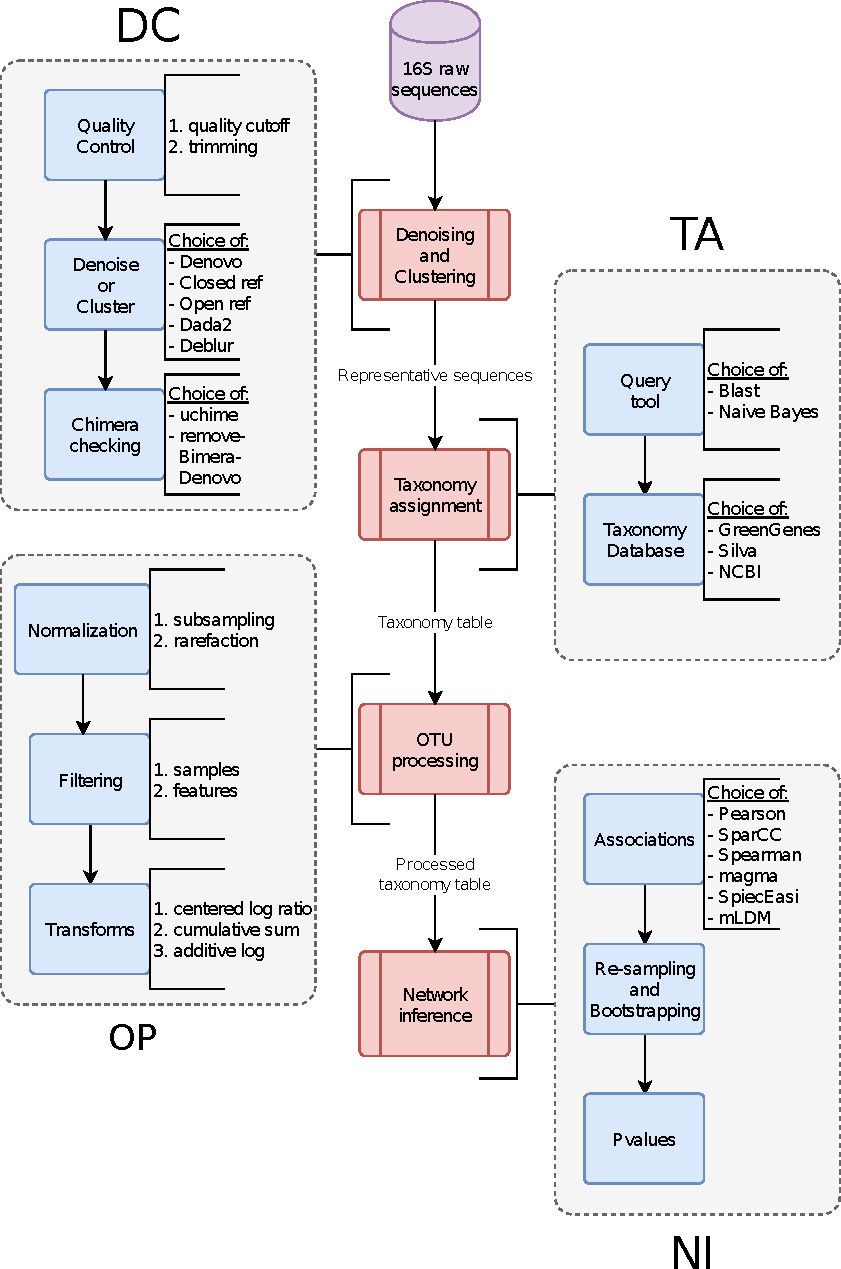
\includegraphics[width=0.74\linewidth]{figure1.pdf}
  % \end{figure}
  \begin{figure}[H]
    \centering
    \caption{
      \textbf{The workflow of the \ac{micone} pipeline}.
      The steps of the workflow can be broken down into five major groups: \textbf{(SP)} \textbf{S}equence \textbf{P}rocessig, \textbf{(DC)} \textbf{D}enoising and \textbf{C}lustering, \textbf{(TA)} \textbf{T}axonomy \textbf{A}ssignment, \textbf{(OP)} \textbf{O}TU and ESV \textbf{P}rocessing, and \textbf{(NI)} \textbf{N}etwork \textbf{I}nference.
      Each step incorporates several processes, each of which in turn have several alternate algorithms for the same task (indicated by the text to the right of the blue boxes).
      The text along the arrows describes the data that is being passed from one step to another.
      The final output of the pipeline is the consensus network generated from the inferred co-occurrence networks.
      For details on each process and the outputs, see Methods.
    }
    \label{fig:figure1}
  \end{figure}



  % \FloatBarrier
  % \newpage
  % \begin{figure}[H]
  %   \centering
  %   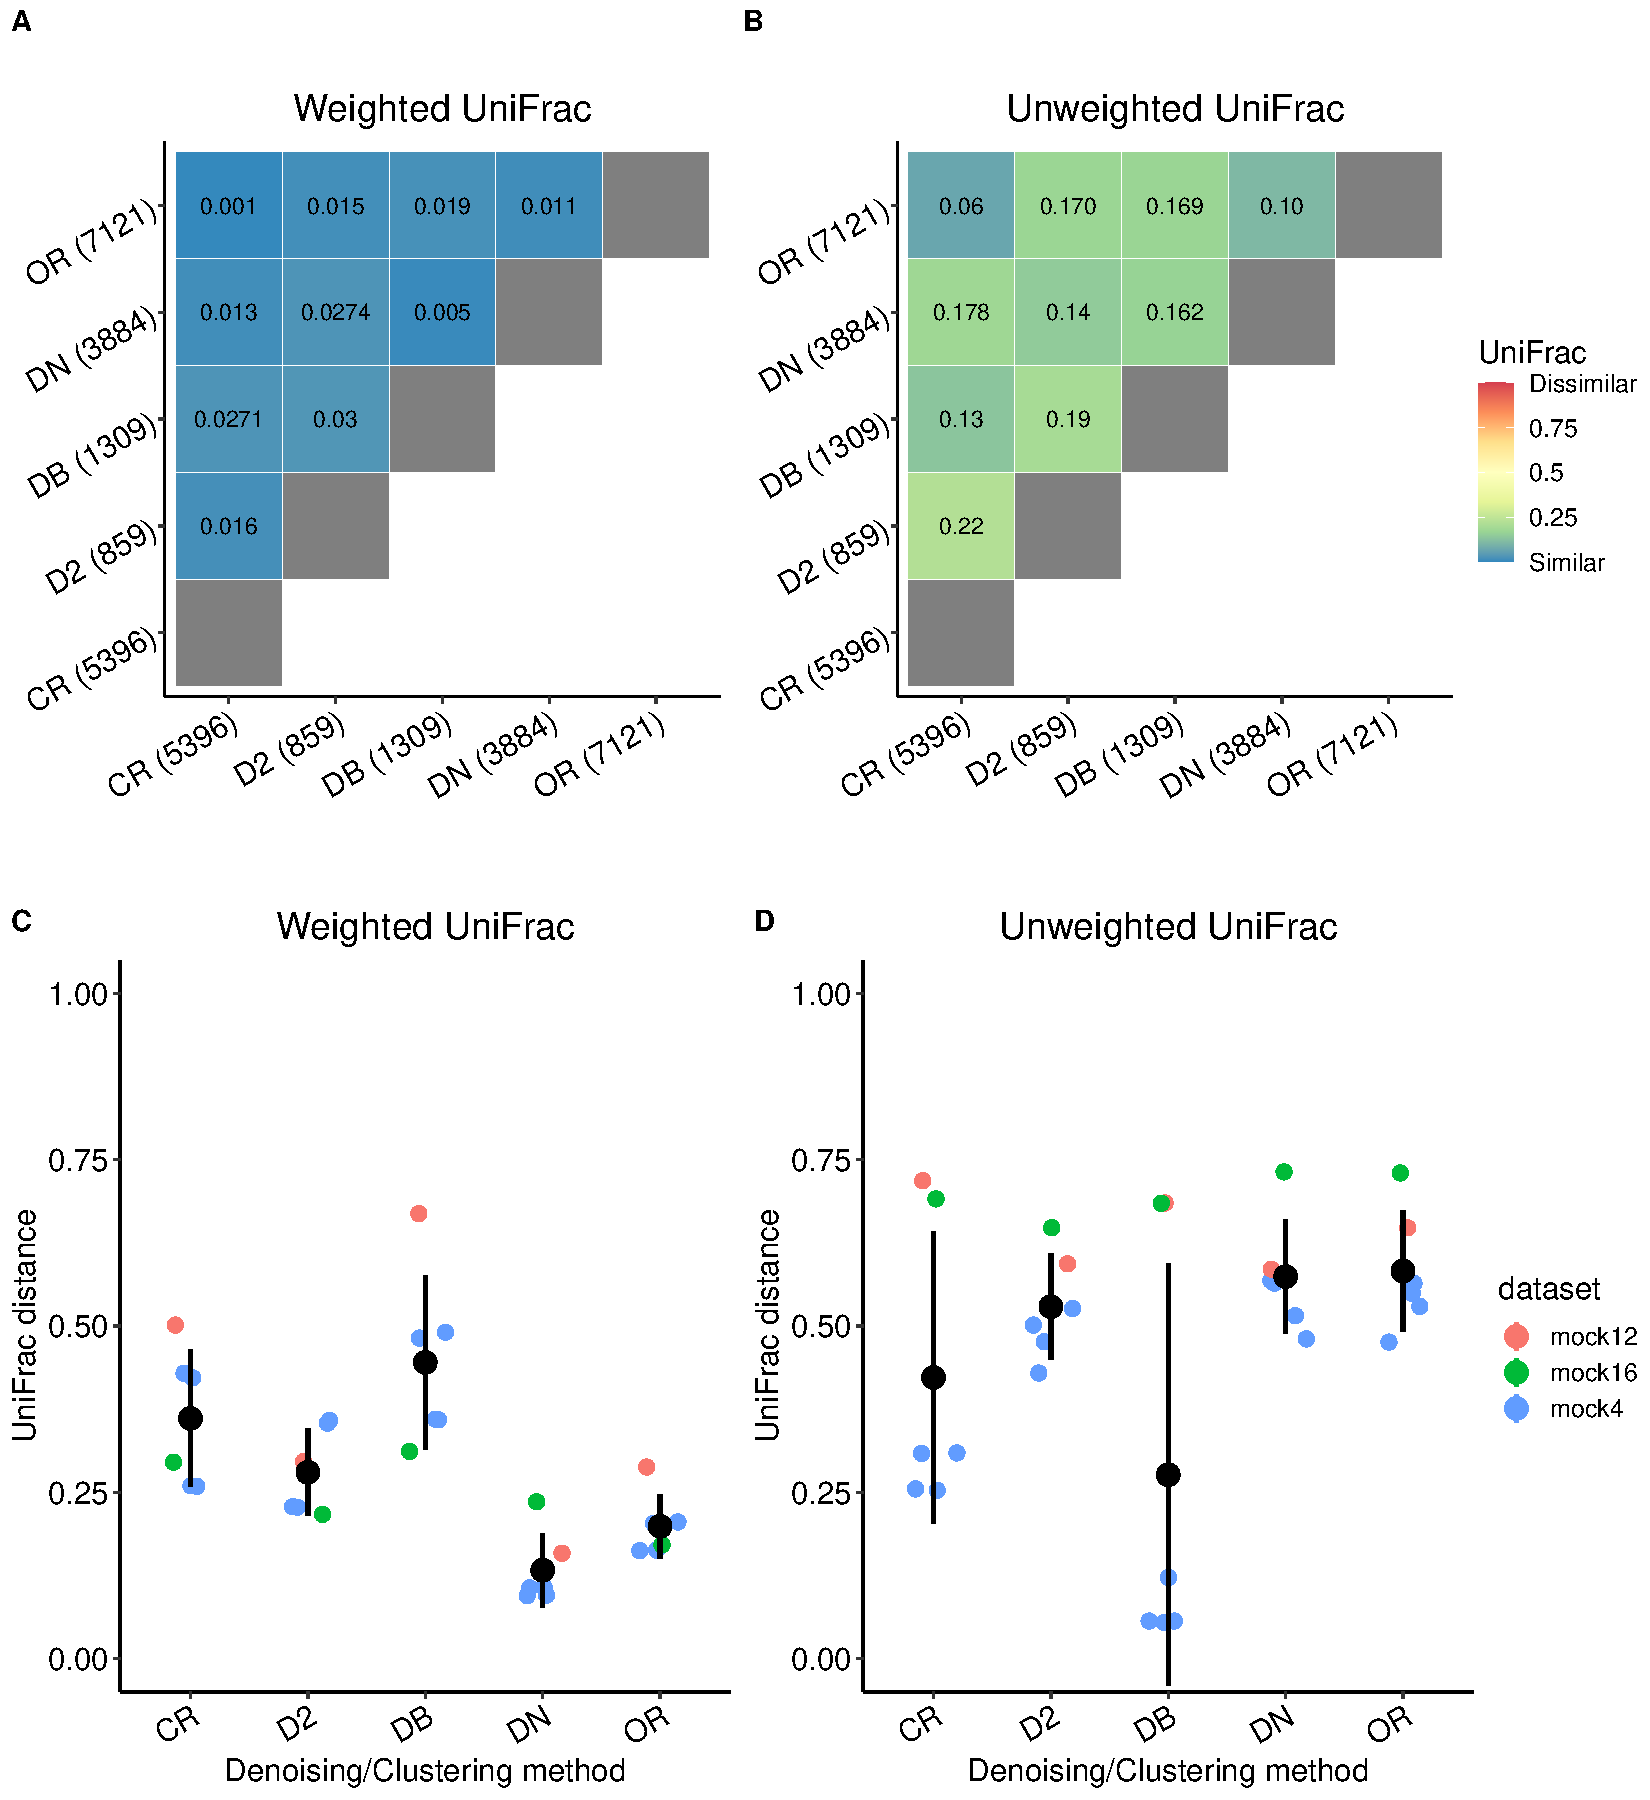
\includegraphics[width=\textwidth]{figure2.pdf}
  % \end{figure}
  \begin{figure}[H]
    \centering
    \caption{
      \textbf{The representative sequences generated by the different DC methods differ in their identification of sequences that are low in abundance.}
      \textbf{(A)} The average weighted UniFrac distance between the representative sequences shows that the representative sequences and their compositions are fairly identical between the methods (with the exception of Deblur (DB)).
      \textbf{(B)} The relatively larger average unweighted UniFrac distance indicates that methods differ in their identification of sequences that are lower in abundance.
      The number of \ac{otu}s or \ac{esv}s generated by the respective methods are provided in the parenthesis next to the names.
      The data used for the analysis in \textbf{(A, B)} were all the samples from the fecal microbiome transplant (FMT) dataset~\cite{Kang2017}, containing both healthy subjects and subjects with autism spectrum disorder (ASD).
      \textbf{(C, D)} The distributions of the average weighted and unweighted UniFrac distance between the expected sequence profile and the predicted sequence profile in the mock datasets.
      The distributions of the average weighted UniFrac distance show that de novo (DN) and open reference (OR) were the best-performing methods in most of the datasets, while they are worst performing methods under the unweighted UniFrac metric.
      The good performance of dada2 (D2) under both distance metrics combined with its approach of identifying \ac{esv}s using de novo methods, prompts us to propose it as the default method for the DC step.
      The data used for the analysis in \textbf{(C, D)} were the mock datasets from mockrobiota~\cite{Bokulich2016}.
    }
    \label{fig:figure2}
  \end{figure}


  % \FloatBarrier
  % \newpage
  % \begin{figure}[H]
  %   \centering
  %   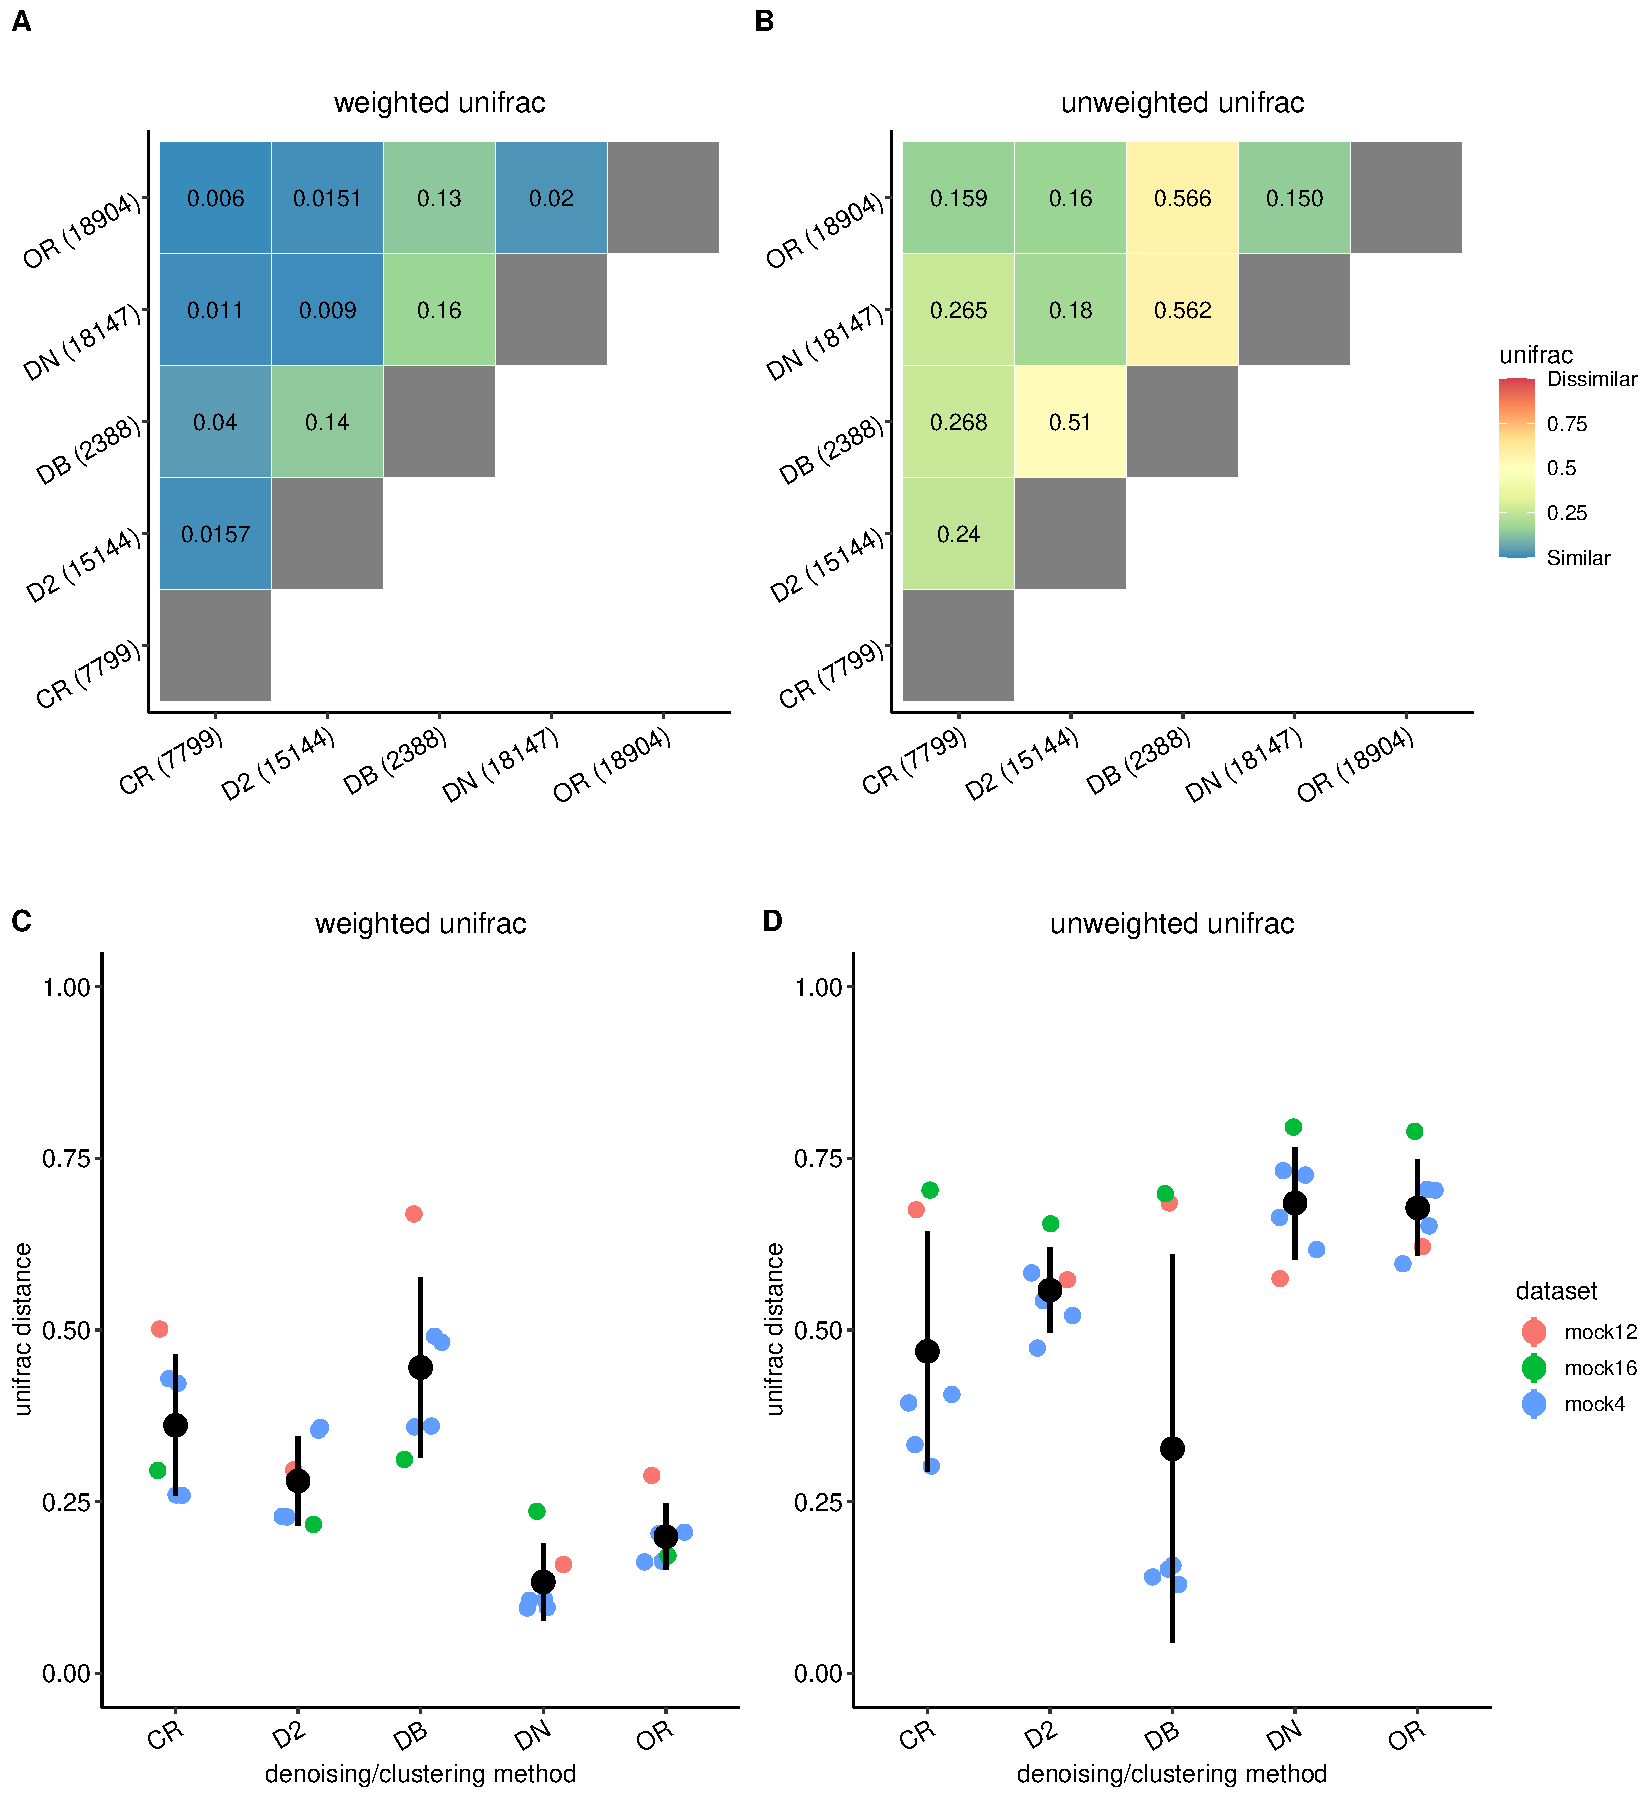
\includegraphics[width=\textwidth]{figure3.pdf}
  % \end{figure}
  \begin{figure}[H]
    \centering
    \caption{
      \textbf{Taxonomic reference databases vary in terms of their taxonomy assignments beyond the Order level.}
      \textbf{(A)} The assignments of the top 50 representative sequences to their respective taxonomies using the three different reference databases.
      This result illustrates how the same sequences are assigned to different Genus under different databases.
      A significant portion of the representative sequences are assigned to an ``unknown'' Genus in two of three databases (\ac{gg} and \ac{ncbi}).
      The number of assigned genera for each database are displayed at the top of each column.
      \textbf{(B)} The number of representative sequences assigned to the same taxonomic label when using different reference databases, shown for the top 100 sequences.
      The number of mismatches are fewer at higher taxonomic levels, but, even at the Order level there exists greater than 51\% of mismatches, demonstrating the poor agreement in taxonomic labels assigned by the different databases.
      The data used for the analysis in \textbf{(A, B)} were all the samples (healthy and ASD) from the FMT dataset.
      \textbf{(C)} The Bray-Curtis dissimilarity between the expected taxonomy profile and calculated taxonomy profile in the mock datasets shows that there is no singular best choice of database for every dataset, as all the databases have similar performance.
      The \ac{gg} database and the Naive Bayes classifier are chosen as the defaults for the TA step of \ac{micone}.
      The datasets used for the analysis in \textbf{(C)} were the mock datasets from mockrobiota.
    }
    \label{fig:figure3}
  \end{figure}


  % \FloatBarrier
  % \newpage
  % \begin{figure}[H]
  %   \centering
  %   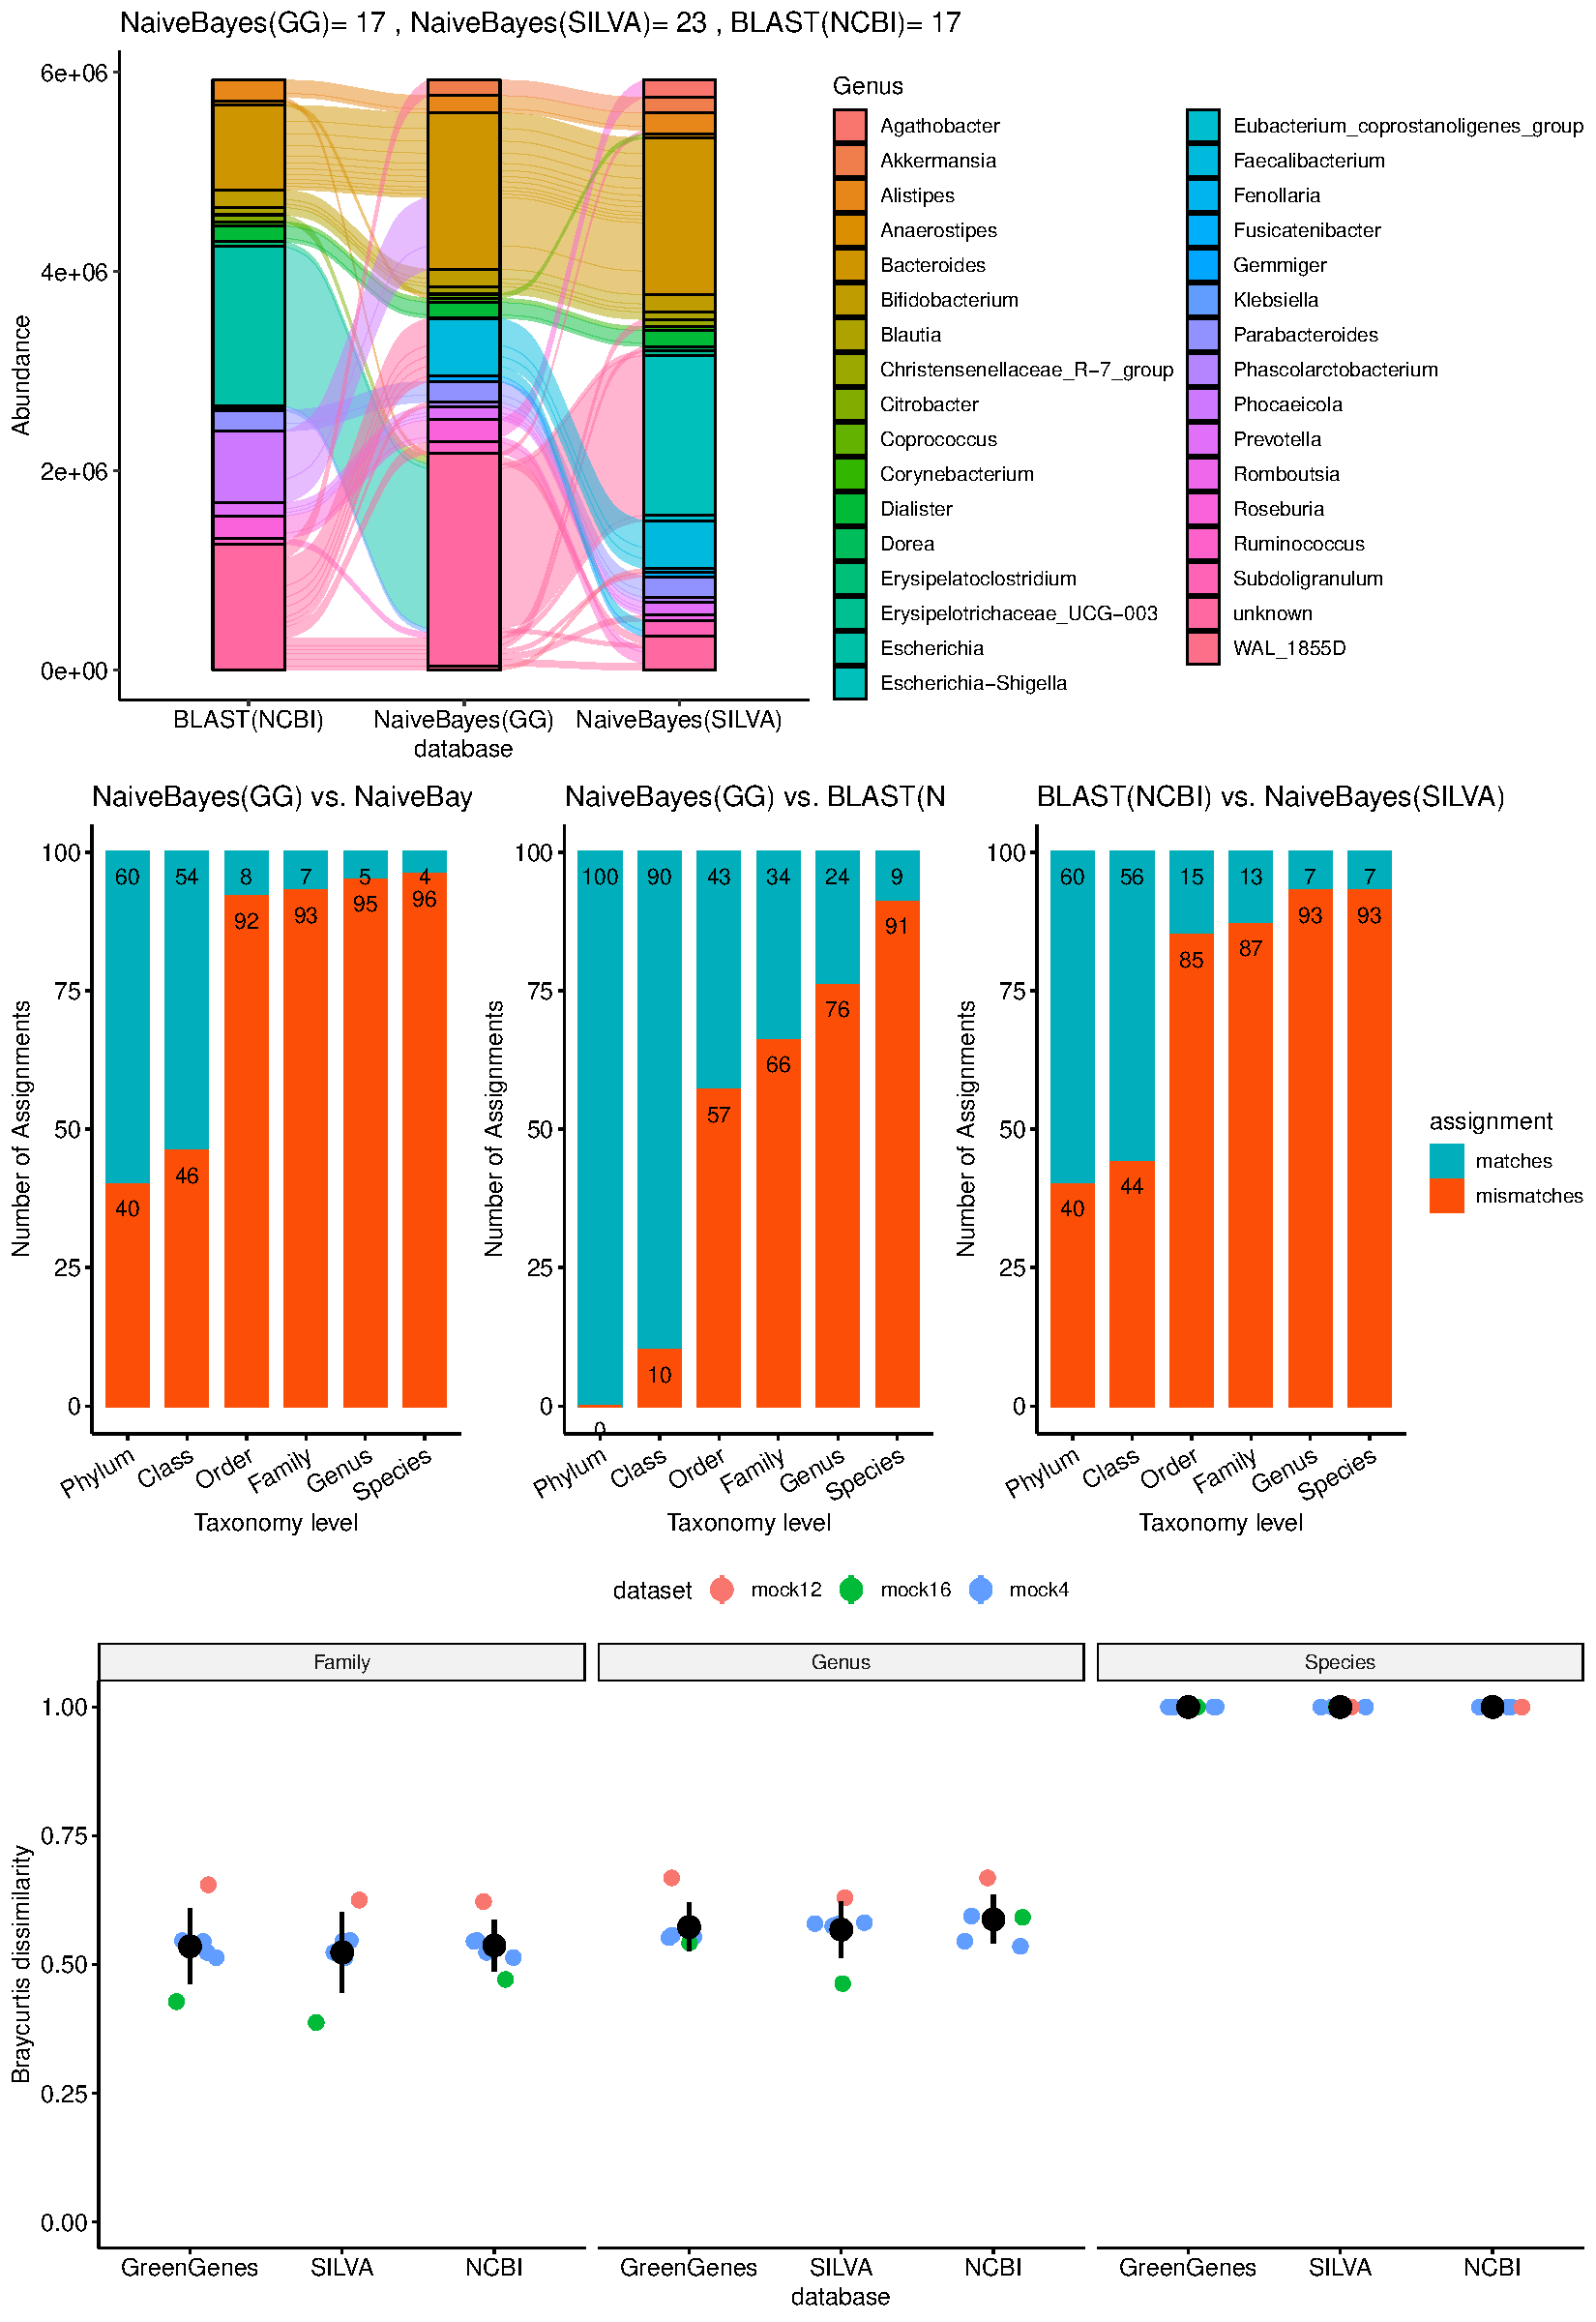
\includegraphics[width=\textwidth]{figure4.pdf}
  % \end{figure}
  \begin{figure}[H]
    \centering
    \caption{
      \textbf{Networks generated using different network inference methods show notable differences both in terms of edge-density and connectivity}.
      \textbf{(A)} The nine different networks (excluding \ac{mldm}) generated by the different network inference methods are very dissimilar.
      The green links are positive associations and the orange links represent negative associations.
      A threshold of 0.3 was set for the correlation-based methods (sparcc, propr, spearman and pearson) and a threshold of 0.01 was set for the direct association methods (flashweave, spieceasi, cozine, harmonies, and spring).
      The correlation-based methods in general produce graph with higher edge-densities.
      \textbf{(B)} The node overlap Upset plot indicates that all the networks have a large proportion of common nodes involved in connections (33 out of 68).
      Whereas, \textbf{(C)} the edge overlap Upset plot shows that a very small fraction of these connections are actually shared (8 out of 202).
      The data used in this analysis were the healthy stool samples from the FMT dataset.
      \ac{mldm} is not shown in the comparisons because the algorithm failed to converge for the particular network combination.
    }
    \label{fig:figure4}
  \end{figure}


  % \FloatBarrier
  % \newpage
  % \begin{figure}[H]
  %   \centering
  %   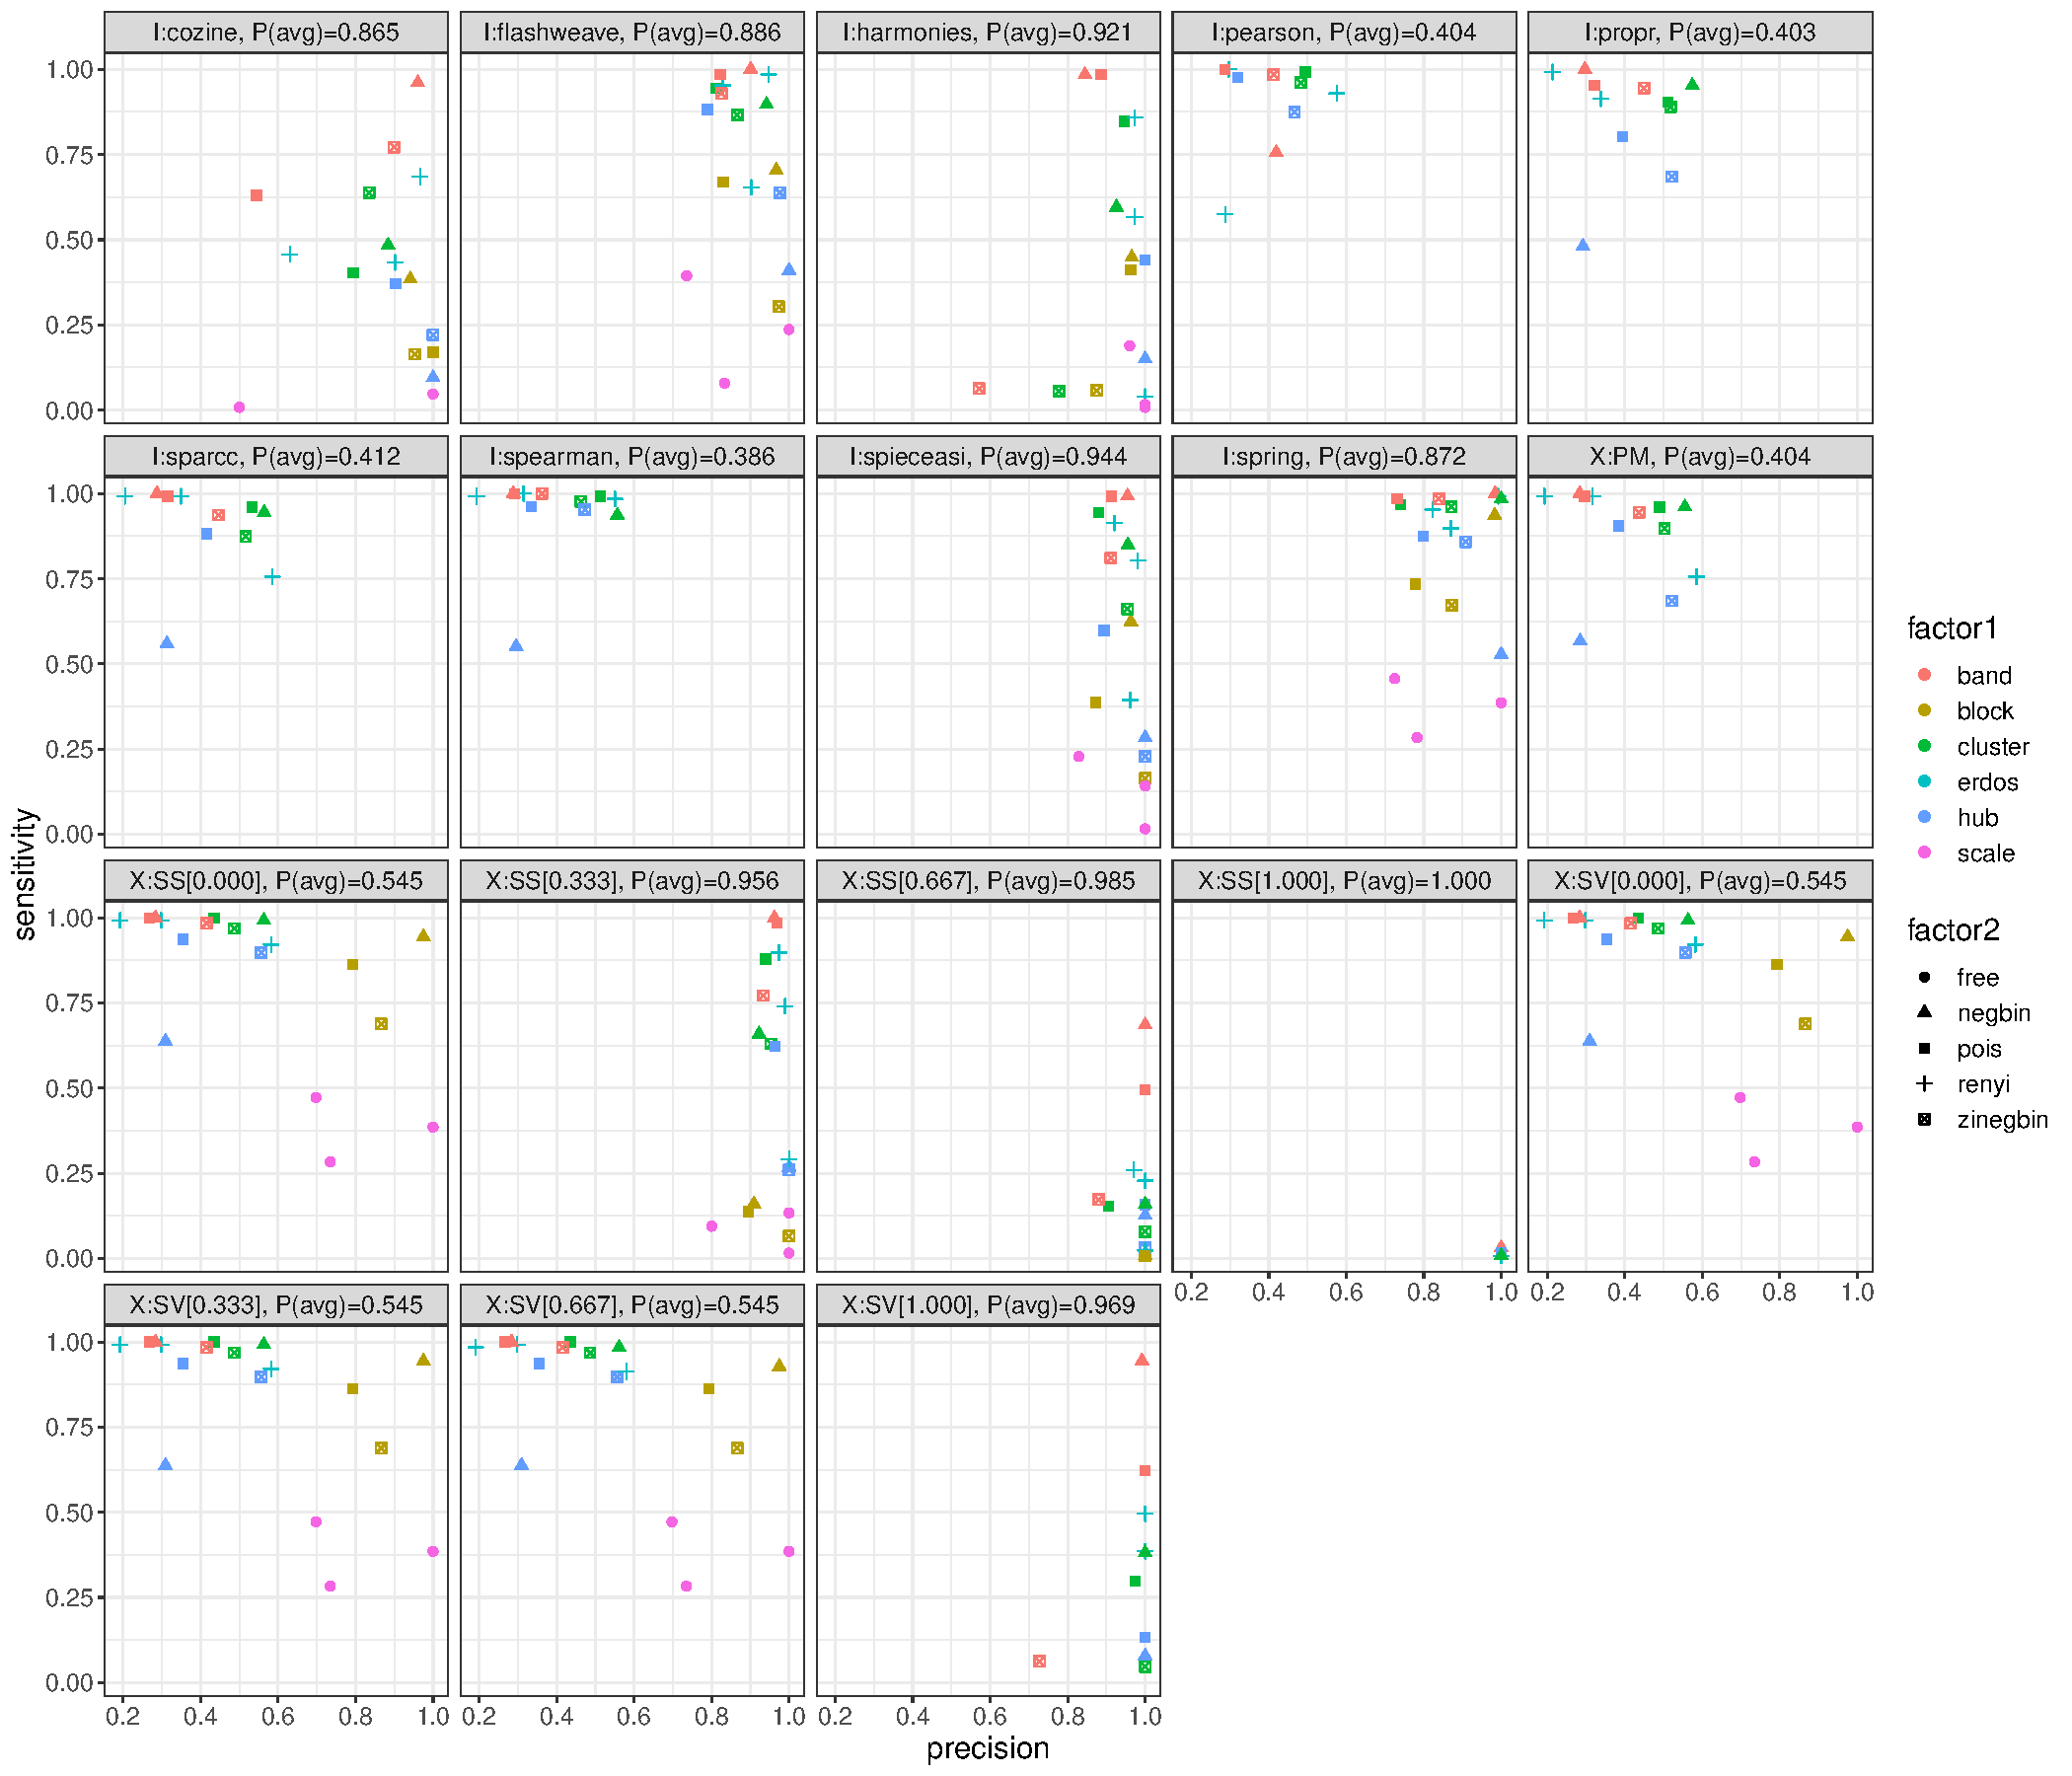
\includegraphics[width=1.0\linewidth]{figure5.pdf}
  % \end{figure}
  \begin{figure}[H]
    \centering
    \caption{
      \textbf{The scaled-sum consensus method returns associations with high precision when applied to the synthetic benchmark datasets}.
      Each point on the box plot shows the precision of the co-occurrence network generated by the individual and consensus methods using the ``NorTA'' and ``seqtime'' methods (refer to Methods).
      The independent algorithms chosen for the comparison are the two best-performing correlation-based (propr, \ac{sparcc}) and direct association based (\ac{spieceasi}, FlashWeave) methods.
      A weight threshold of 0.1 and a p-value threshold of 0.05 was applied to each network before the calculation of precision.
      The different consensus based methods used are the scaled-sum (SS) and simple voting (SV) method.
      The overall best precision was consistently obtained by the scaled-sum method for $p \geq 0.333$ on both datasets.
      Among all the independent network inference methods, \ac{spieceasi} has the best average precision.
      The simple voting method when using presence of edges in all inferred networks as a requirement ($p = 1.000$), also outperforms \ac{spieceasi} on average precision.
      Therefore, we recommend the scaled-sum consensus method with $p = 0.333$ as the default tool for network inference, as this option provides a good balance of precision and sensitivity.
    }
    \label{fig:figure5}
  \end{figure}


  % \FloatBarrier
  % \newpage
  % \begin{figure}[H]
  %   \centering
  %   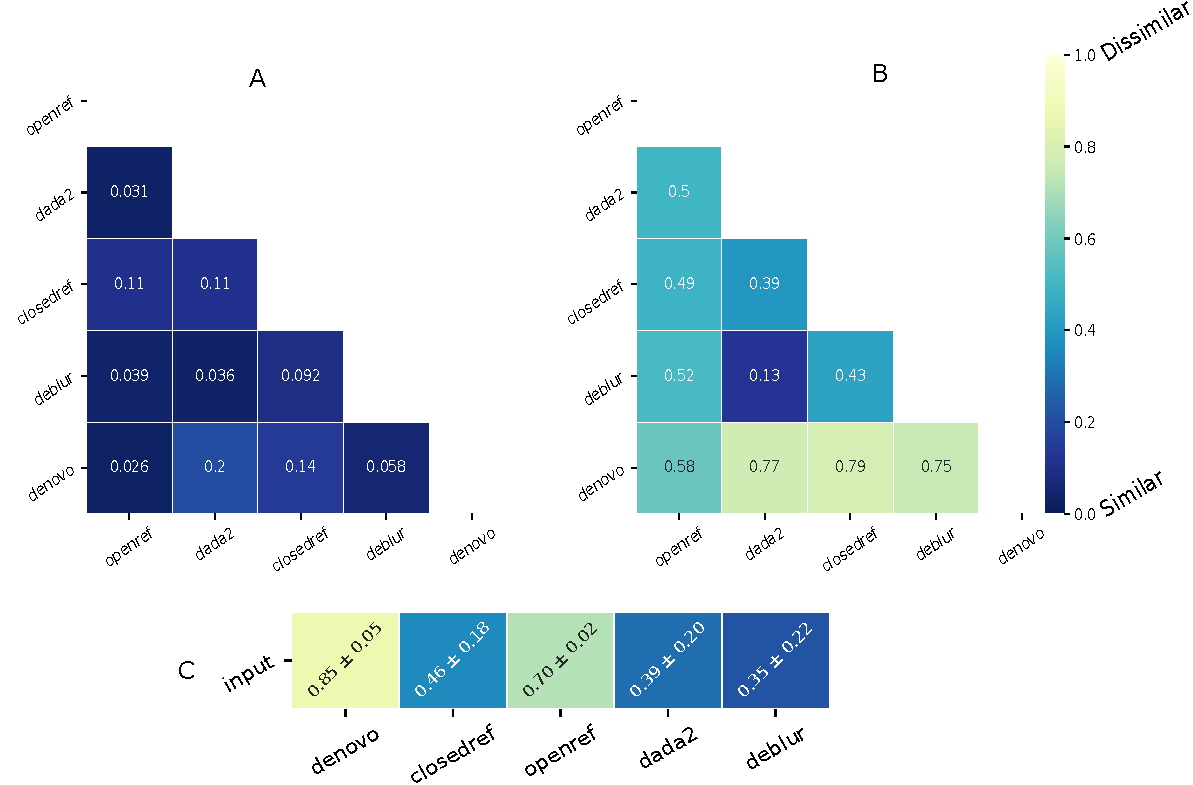
\includegraphics[width=\textwidth]{figure6.pdf}
  % \end{figure}
  \begin{figure}[H]
    \centering
      \caption{
      \textbf{The choice of reference database contributes has the largest impact on network variance}.
      \textbf{(A)} The percentage of variance in the networks contributed by the DC, CC (chimera checking), TA, OP and NI steps of the pipeline calculated using ANOVA on the linear model, see the Methods section for details.
      The data used for the analysis were the healthy stool samples from the FMT dataset.
      A weight threshold of 0.1 and a p-value threshold of 0.05 was applied to each network before the analysis.
      The taxonomy database contributes most to the variance between the networks (65.4\%) followed by the filtering of the counts matrix (26.8\%) in the OP step.
    The variation due to the DC and CC steps are much smaller in comparison (0.648\% and 0.003\% respectively).
      The fraction labeled as the residual is an artifact that arises when multiple steps are changed at the same time, however, this can be ignored as this fraction is negligible.
      \textbf{(B)} All combinations of inferred networks are shown as points on a PCA plot.
      Each point on the PCA plot represents a network inferred using different combinations of tools and parameters that are available in the \ac{micone} pipeline.
      The color of the points corresponds to the tools used at each step of the pipeline (DC, TA, OP and NI).
      The points on the PCA plot can be grouped based on the TA step, but at the NI step only some methods create high variability in the inferred networks.
      The \ac{dc} step does not seem to have any correlation with the similarity of networks on the PCA plot, but all the networks with filtering at the \ac{op} step are similar to each other.
      This further confirms that the variability in the networks decreases upon filtering out the taxonomic entities at low abundance.
    }
    \label{fig:figure6}
  \end{figure}


  % \FloatBarrier
  % \newpage
  % \begin{figure}[H]
  %   \centering
  %   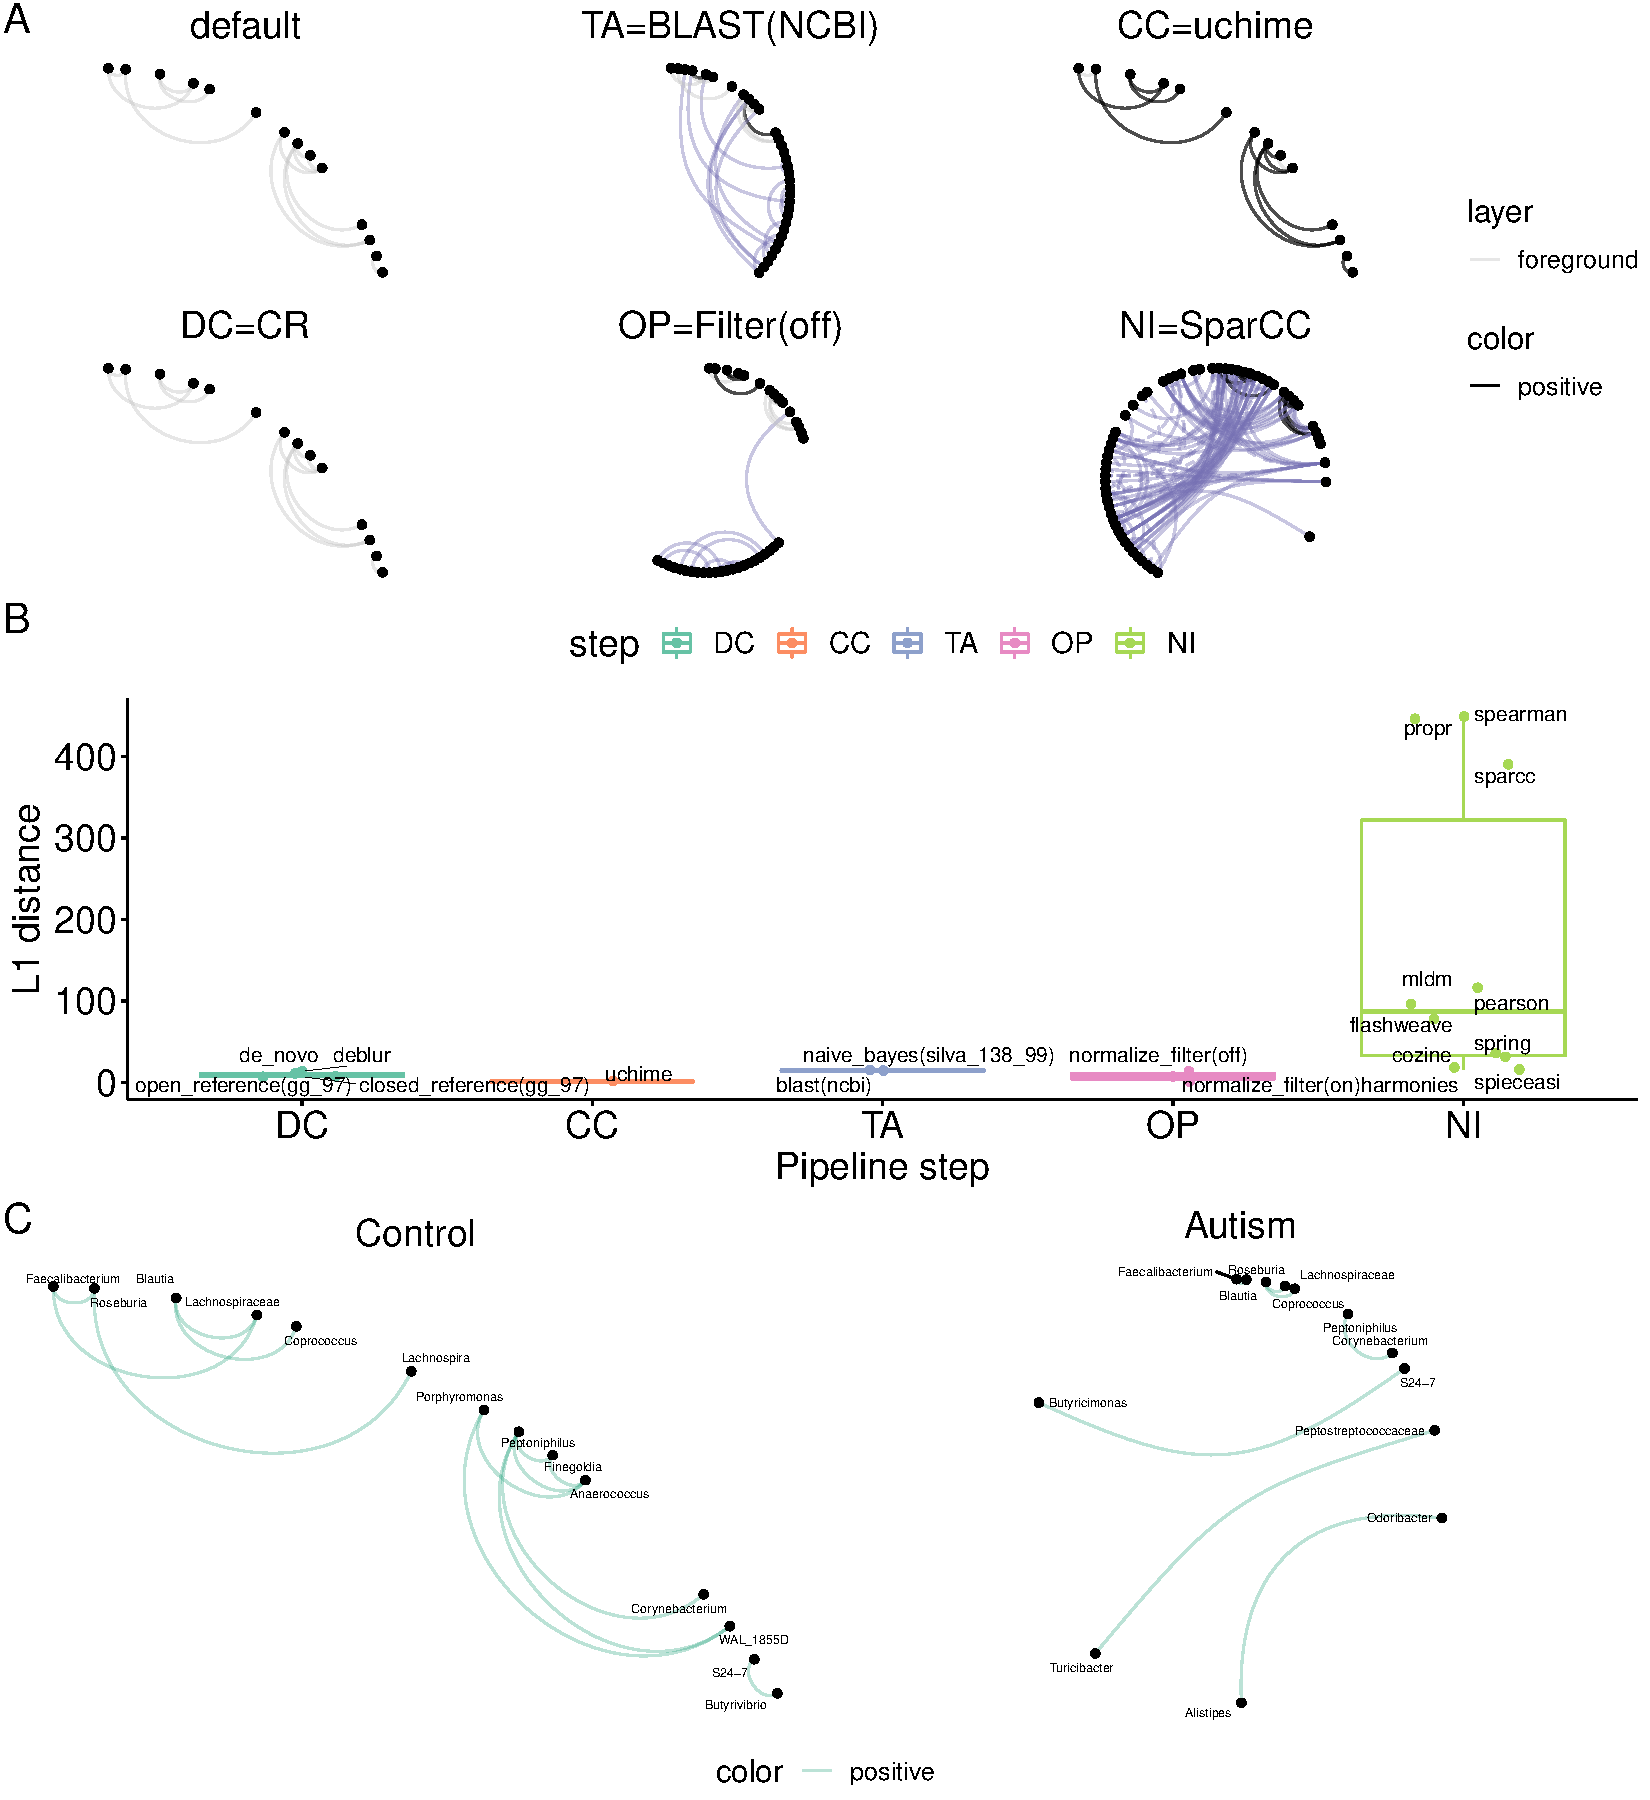
\includegraphics[width=1.0\linewidth]{figure7.pdf}
  % \end{figure}
  \begin{figure}[H]
    \centering
    \caption{
      \textbf{Comparison of networks generated from control and ASD samples using the \ac{micone} pipeline}.
      The networks for the control (left) and ASD (right) samples in the FMT dataset were generated using the default tools and parameters recommended by the \ac{micone} pipeline.
      There are 20 unique links in the network for control samples, 12 unique links in the network for ASD subjects and 7 edges in common between both networks.
    }
    \label{fig:figure7}
  \end{figure}


  \FloatBarrier
  \newpage
  \subsection*{Supplementary tables and figures}
  
  \renewcommand{\thefigure}{S\arabic{figure}}
  \setcounter{figure}{0}

  \renewcommand{\thetable}{S\arabic{table}}
  \setcounter{table}{0}


    % \begin{figure}[H]
    %   \centering
    %   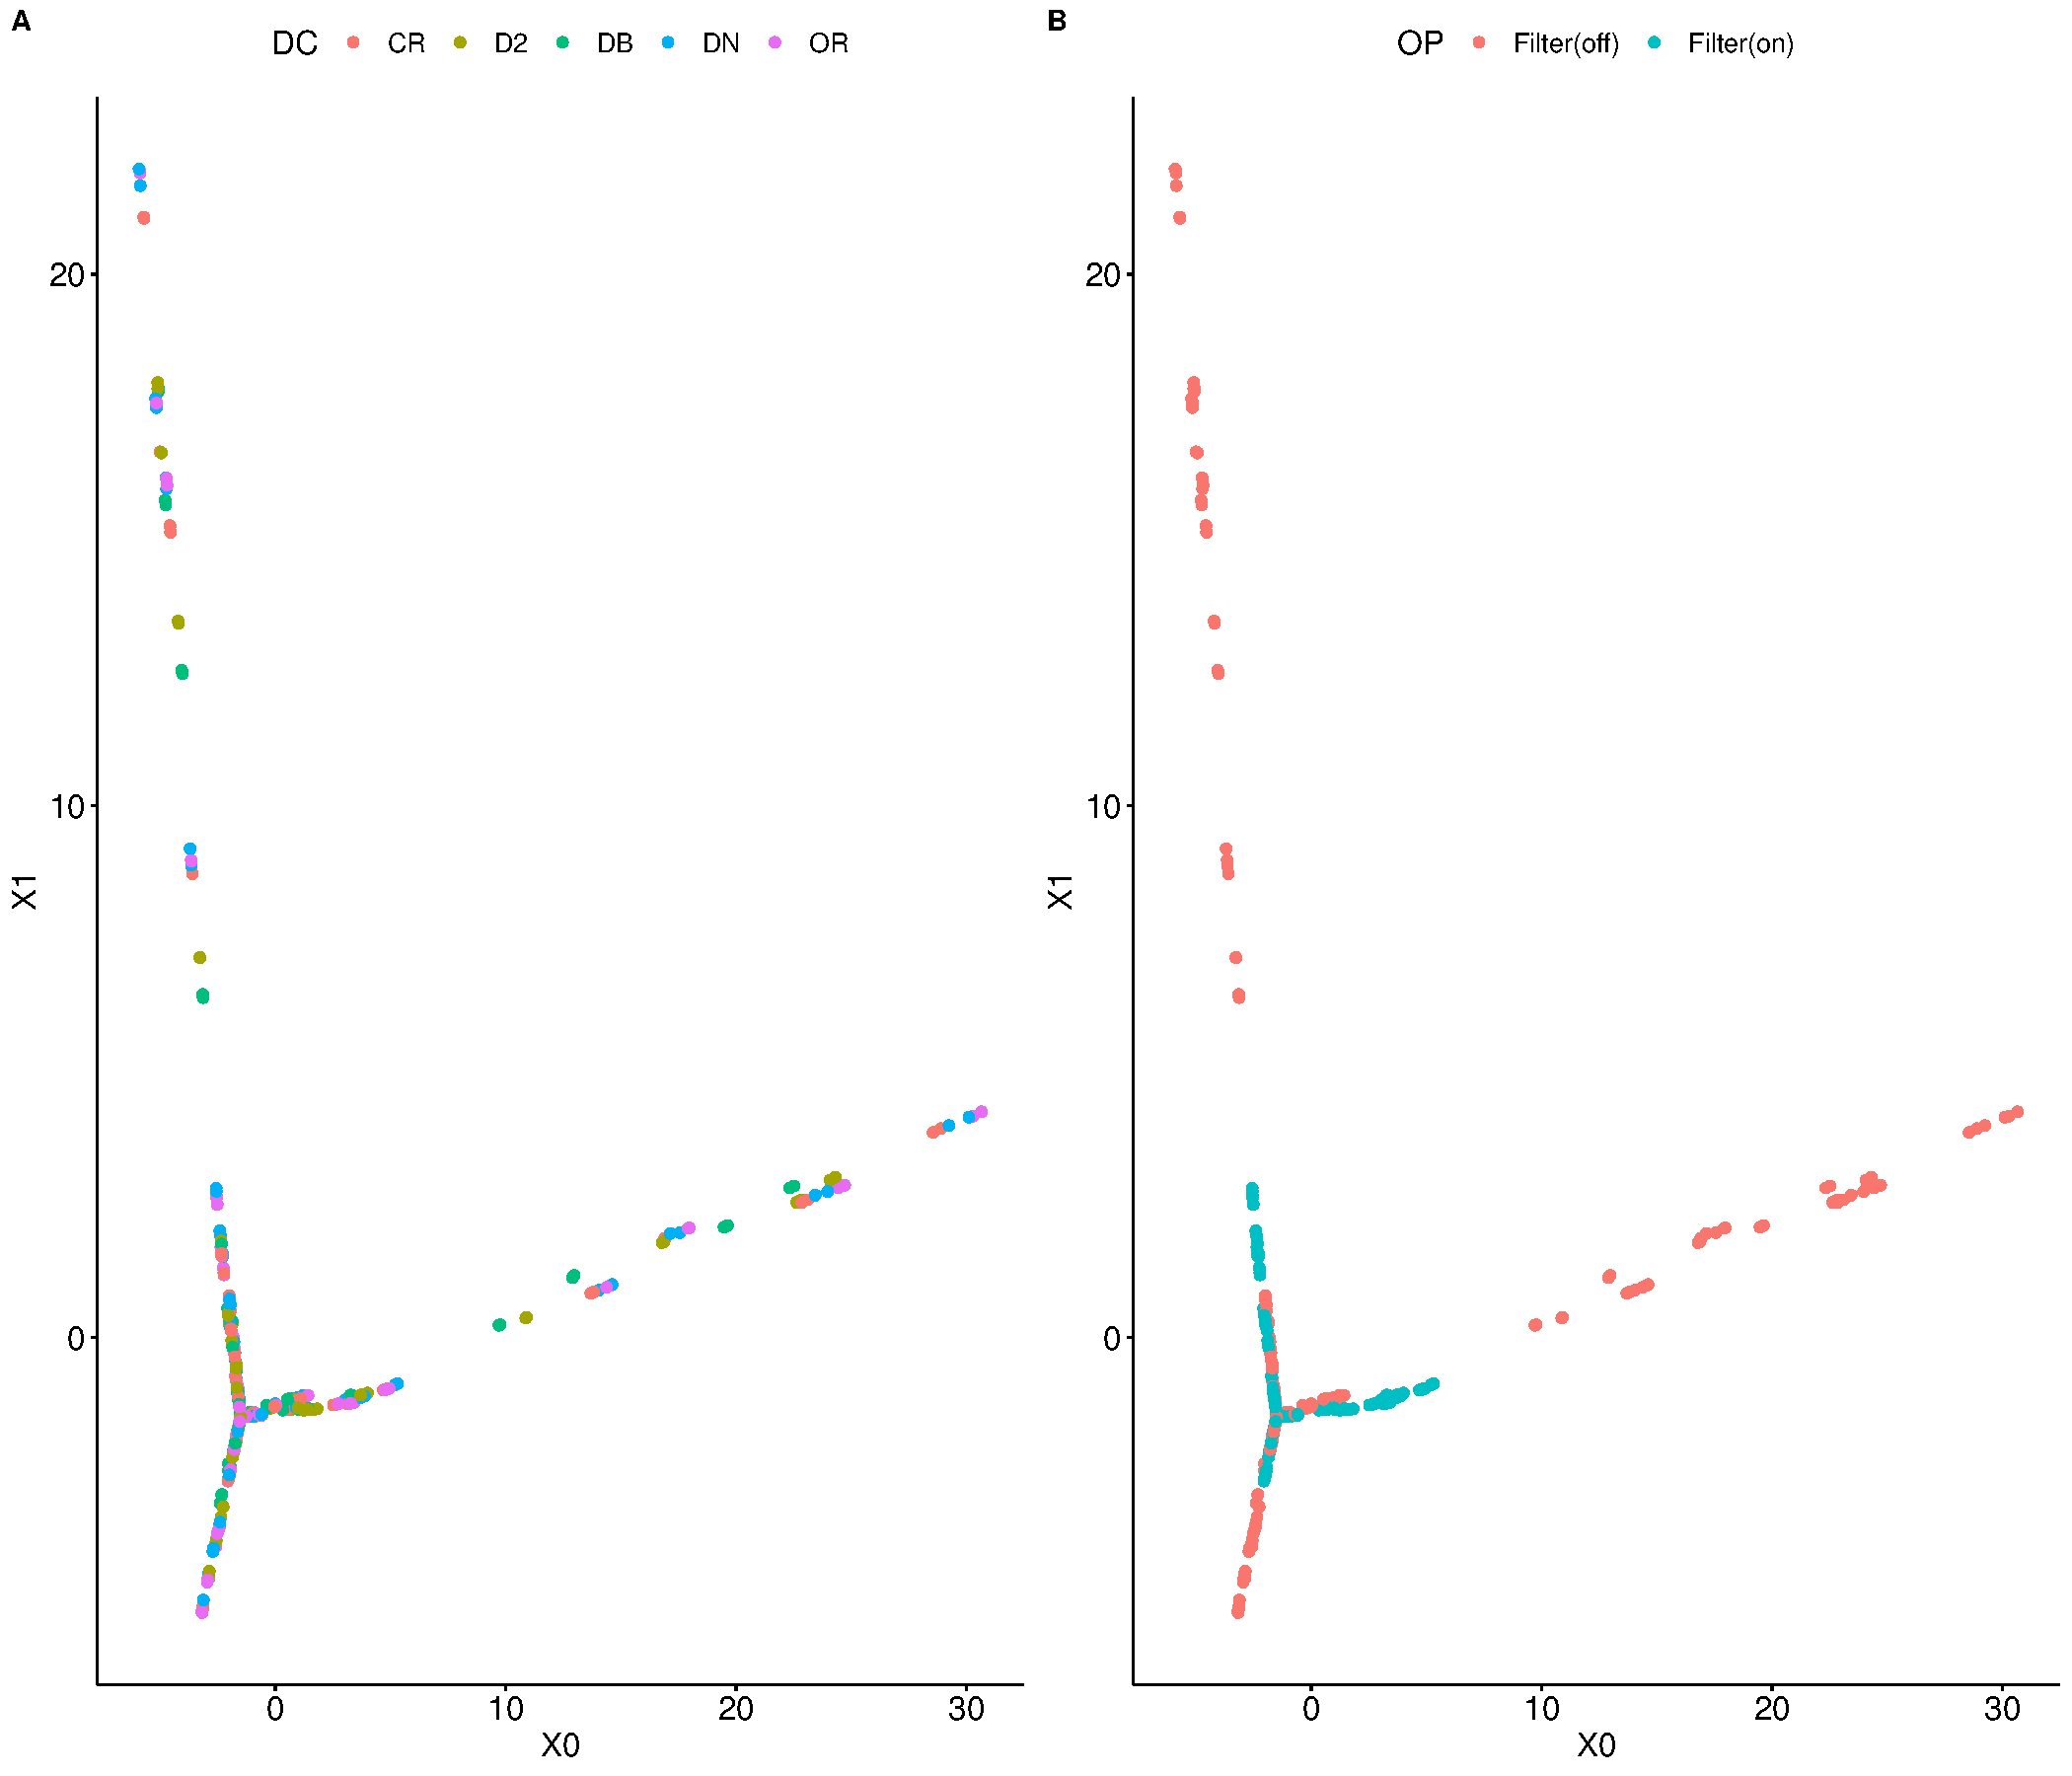
\includegraphics[width=1.0\linewidth]{figure_s1.pdf}
    % \end{figure}
    \begin{figure}[H]
      \centering
        \caption{
          \textbf{The t-SNE plot of all the inferred networks clusters the networks based on the taxonomy reference database used}.
          Each point on the t-SNE plot represents a network inferred using different combinations of tools and parameters that are available in the \ac{micone} pipeline.
          The points are colored by the tools and parameters used in \ac{dc} step (A), \ac{ta} step (B), \ac{op} step (C) and \ac{ni} step (D).
          The separation of the points based on taxonomy reference database shows that the points cluster based on reference database in high-dimensional space.
        }
      \label{fig:figure_s1}
    \end{figure}
    % \FloatBarrier
    % \newpage

    % \begin{figure}[H]
    %   \centering
    %   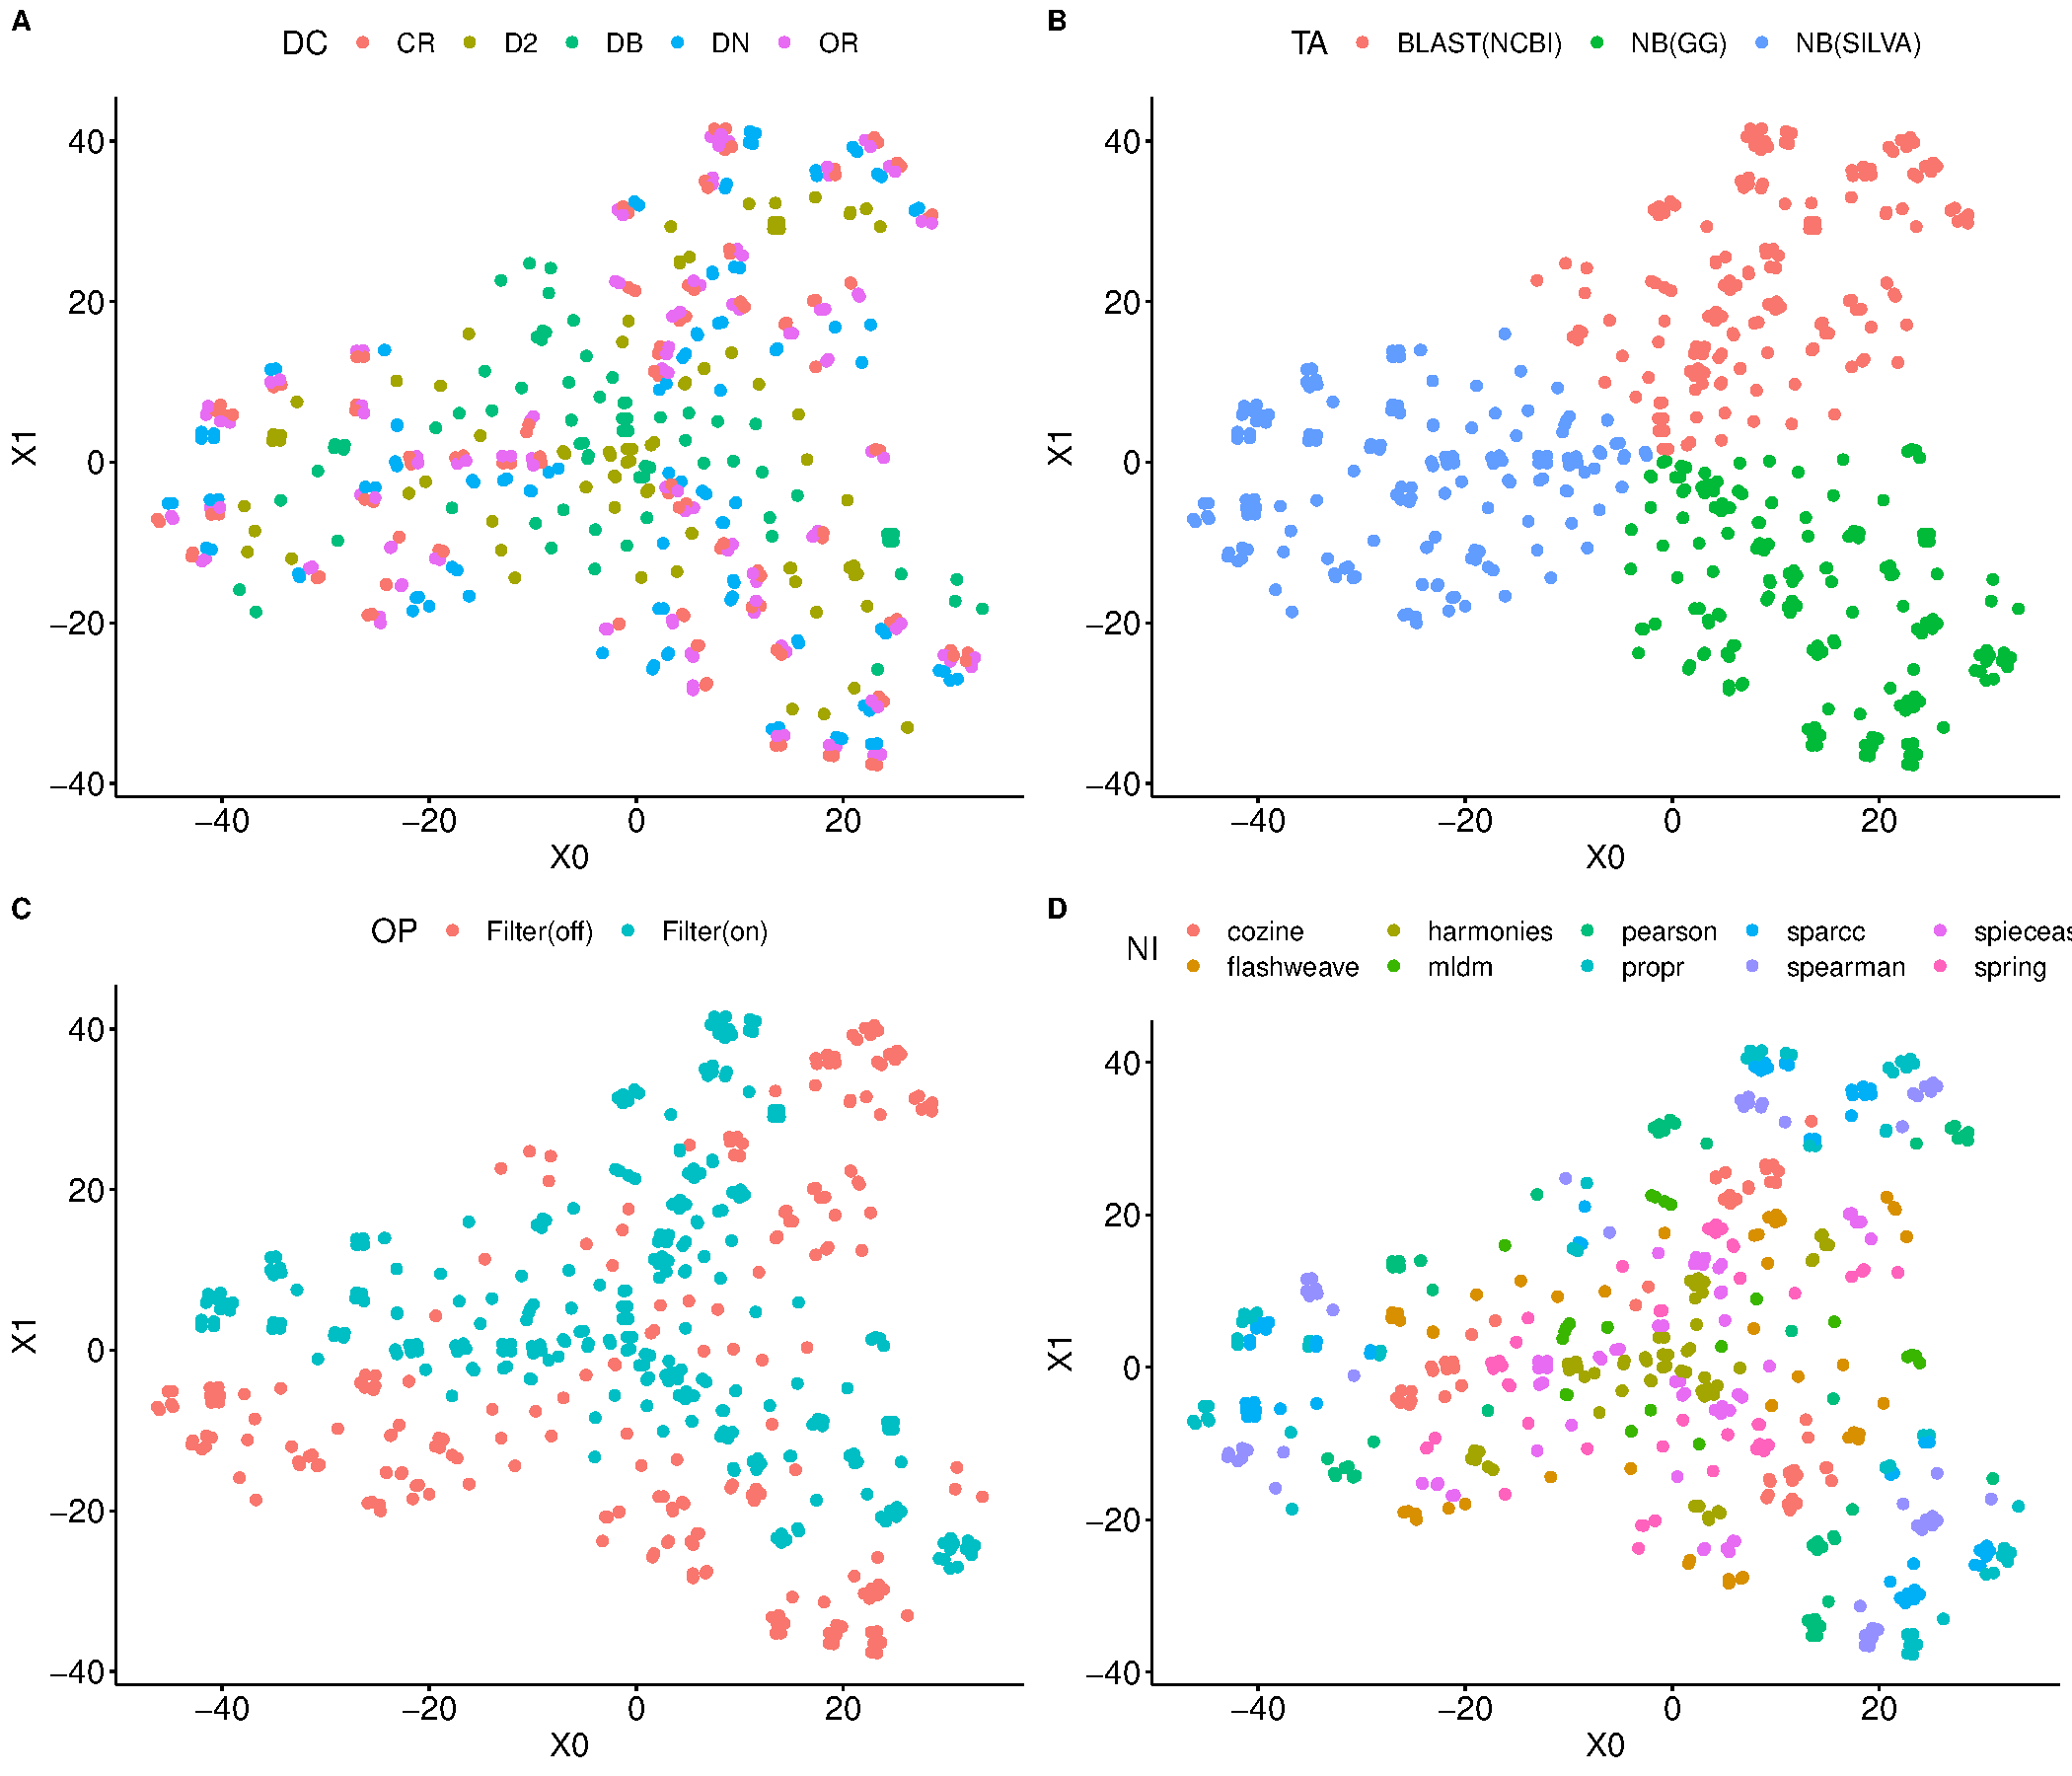
\includegraphics[width=1.0\linewidth]{figure_s2.pdf}
    % \end{figure}
    \begin{figure}[H]
      \centering
        \caption{
          \textbf{The UniFrac distance between the 1000 most abundant representative sequences is higher than that when all sequences are considered}.
          Each value is the average UniFrac distance between the reference sequences generated by the various methods in the \ac{dc} step (similar to Figure~\ref{fig:figure2}).
          There is an increase in both weighted and unweighted UniFrac distances compared to when all the representative sequences are considered.
          This shows that the 1000 most abundant representative sequences generated by the methods are not as similar to each other.
          And since the weighted UniFrac is much smaller than the unweighted UniFrac distance, we can conclude that those reference sequences that are present in the middle of the abundance distribution are dissimilar.
        }
      \label{fig:figure_s2}
    \end{figure}
    % \FloatBarrier
    % \newpage

    % \begin{figure}[H]
    %   \centering
    %   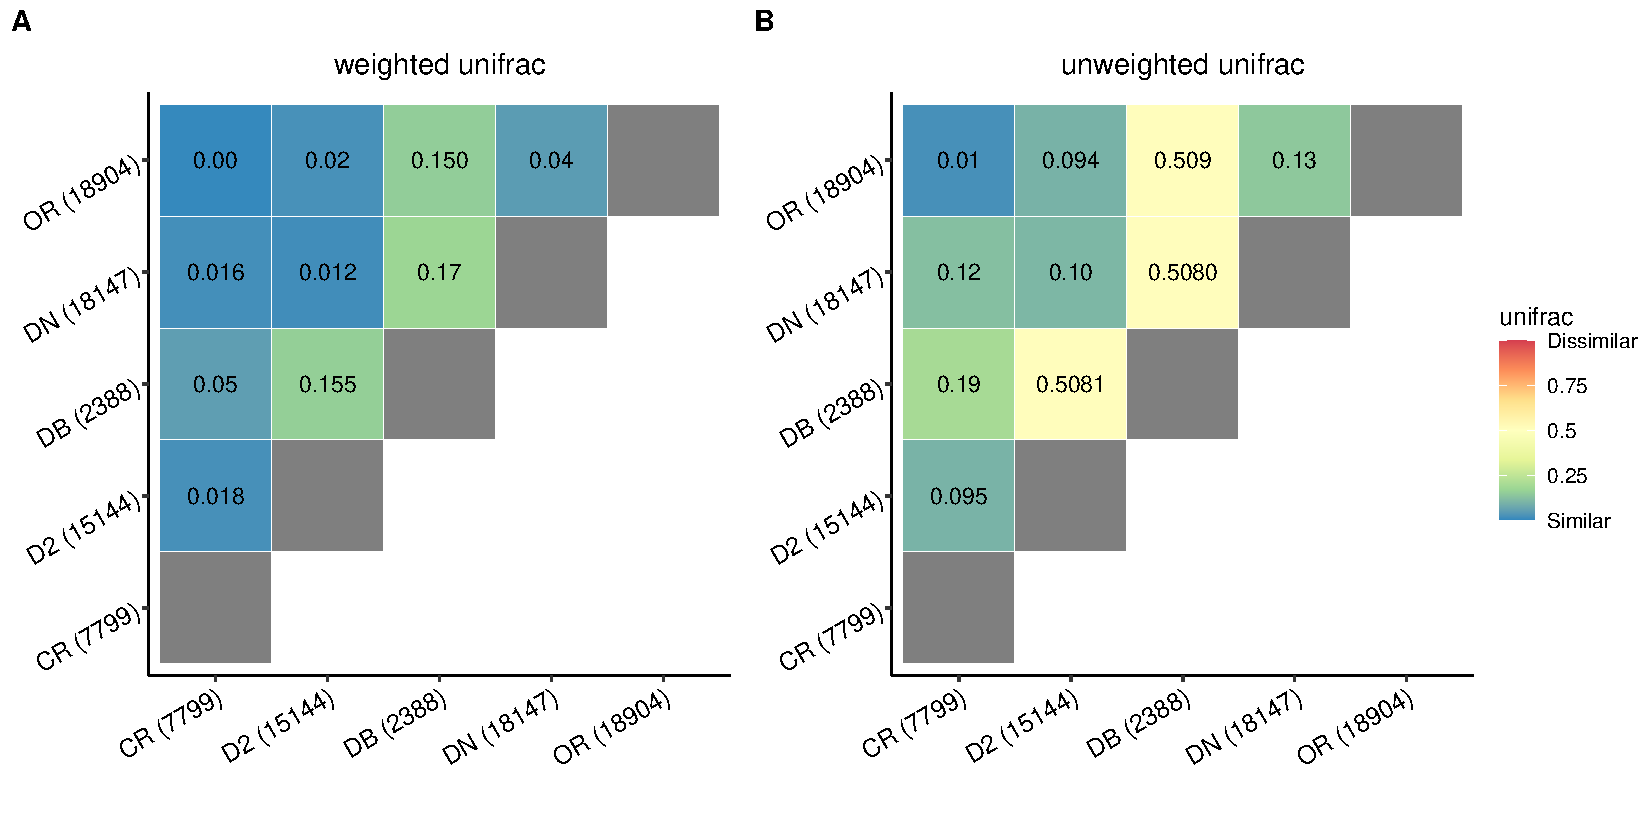
\includegraphics[width=1.0\linewidth]{figure_s3.pdf}
    % \end{figure}
    \begin{figure}[H]
      \centering
        \caption{
          \textbf{The weighted and unweighted UniFrac distances between representative sequences generated using remove bimera and uchime for each denoising method are low.}
          The two chimera checking methods, uchime and remove bimera, produce similar outputs.
          With the exception of de novo and open reference under the unweighted UniFrac metric, all the other methods have low dissimilarity.
          This is especially true for the \ac{dada2} and Deblur methods which are the recommended denoising methods in the \ac{micone} pipeline.
          Therefore, remove bimera is recommended as the default chimera method if one is using \ac{dada2} and uchime-denovo when one is using Deblur, since these methods were developed for these respective algorithms (\ac{qiime2} uses uchime-denovo in the Deblur workflow).
        }
      \label{fig:figure_s3}
    \end{figure}
    % \FloatBarrier
    % \newpage

    % \begin{figure}[H]
    %   \centering
    %   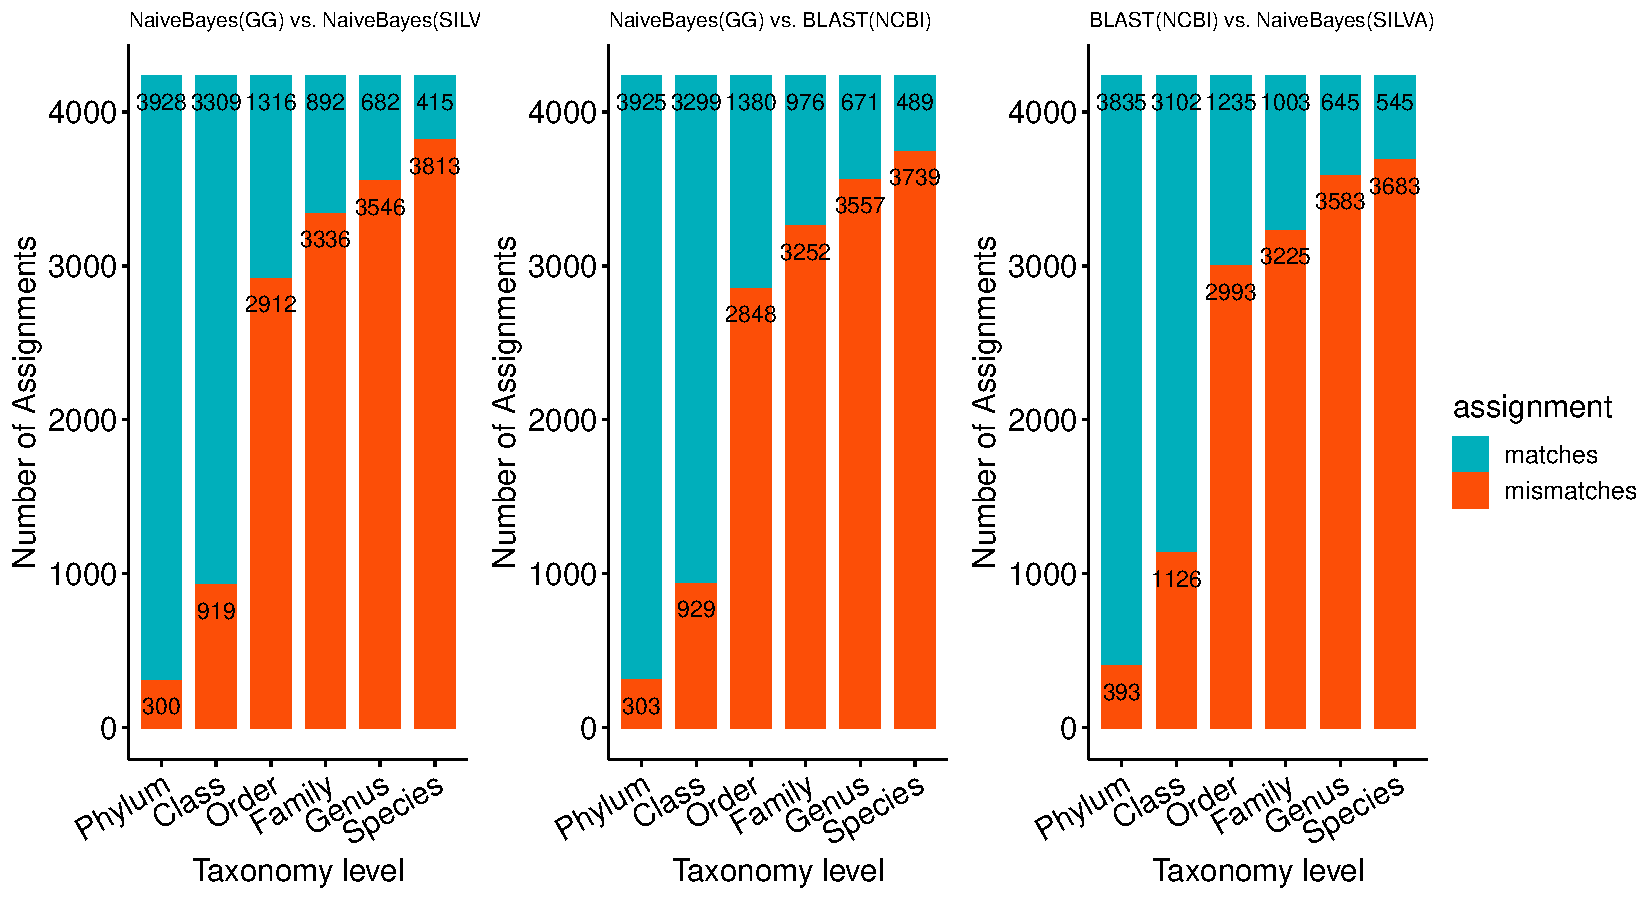
\includegraphics[width=1.0\linewidth]{figure_s4.pdf}
    % \end{figure}
    \begin{figure}[H]
      \centering
        \caption{
          \textbf{The pairwise comparison of assignments generated using different databases for all representative sequences has a higher proportion of mismatches}.
          The comparison made here is similar to Figure~\ref{fig:figure3}B, but instead of the top 100 taxonomic entities (by abundance), all the assignments from one database are matched with those from the other two databases.
          Higher percentage of mismatches implies that the matching of the taxonomies in the more abundant sequences (top 100) are more consistent.
        }
      \label{fig:figure_s4}
    \end{figure}
    % \FloatBarrier
    % \newpage

  % \begin{figure}[H]
  %   \centering
  %   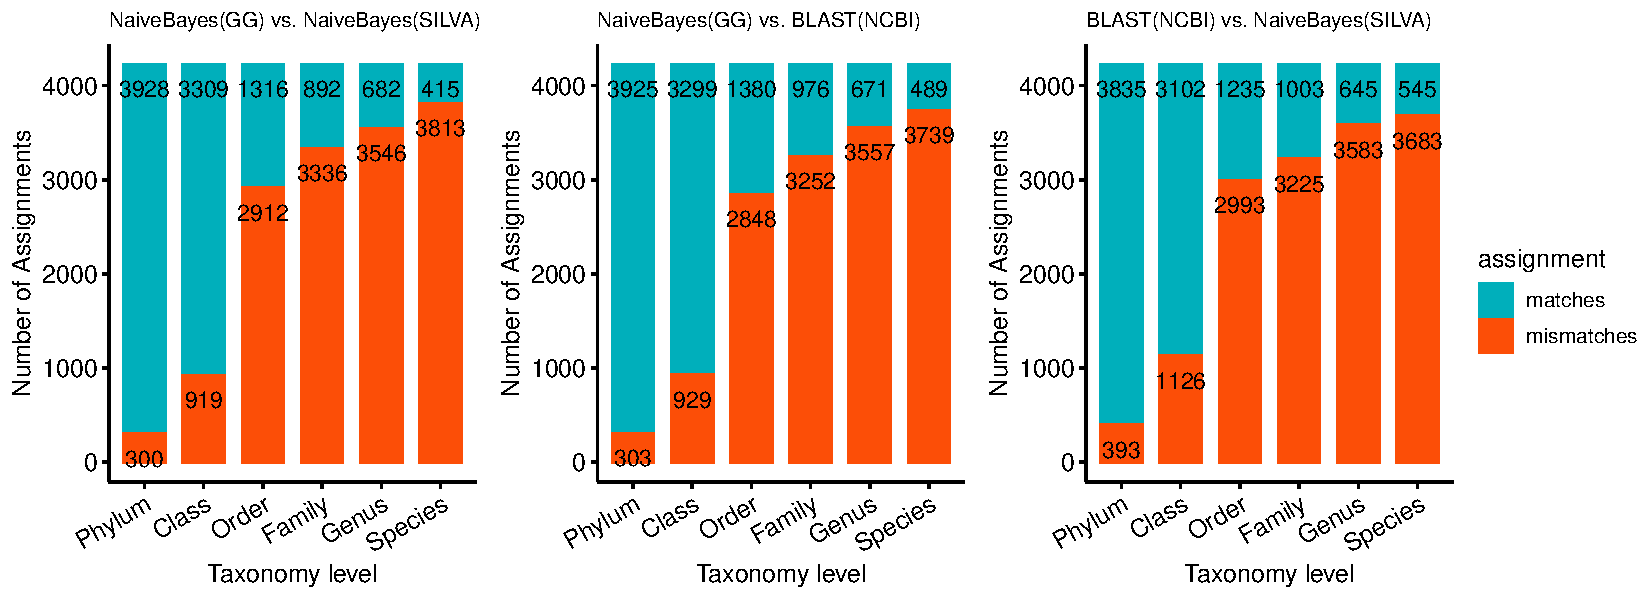
\includegraphics[width=1.0\linewidth]{figure_s5.pdf}
  % \end{figure}
  \begin{figure}[H]
    \centering
      \caption{
        \textbf{The precision and sensitivity of the inferred networks on the ``NorTA'' synthetic interaction data.}
        The different consensus based methods used are: scaled-sum (SS) and simple voting (SV) method.
        Pearson and Spearman methods are not used in the calculation of the consensus.
        Among all the independent network inference methods, \ac{spieceasi} has the best average precision (0.944), but the overall best precision was consistently obtained by the scaled-sum method (0.956, 0.985 and 1.000).
        The simple voting method when using presence of edges in all inferred networks as a requirement ($p = 1.000$), also outperforms \ac{spieceasi} on average precision (0.969).
        Although \ac{spieceasi} has a higher performance on sensitivity, if the goal of network inference is to obtain the list of associations that have a high probability of existing in the real microbial community, then the consensus methods perform better.
      }
    \label{fig:figure_s5}
  \end{figure}
  % \FloatBarrier
  % \newpage

  % \begin{figure}[H]
  %   \centering
  %   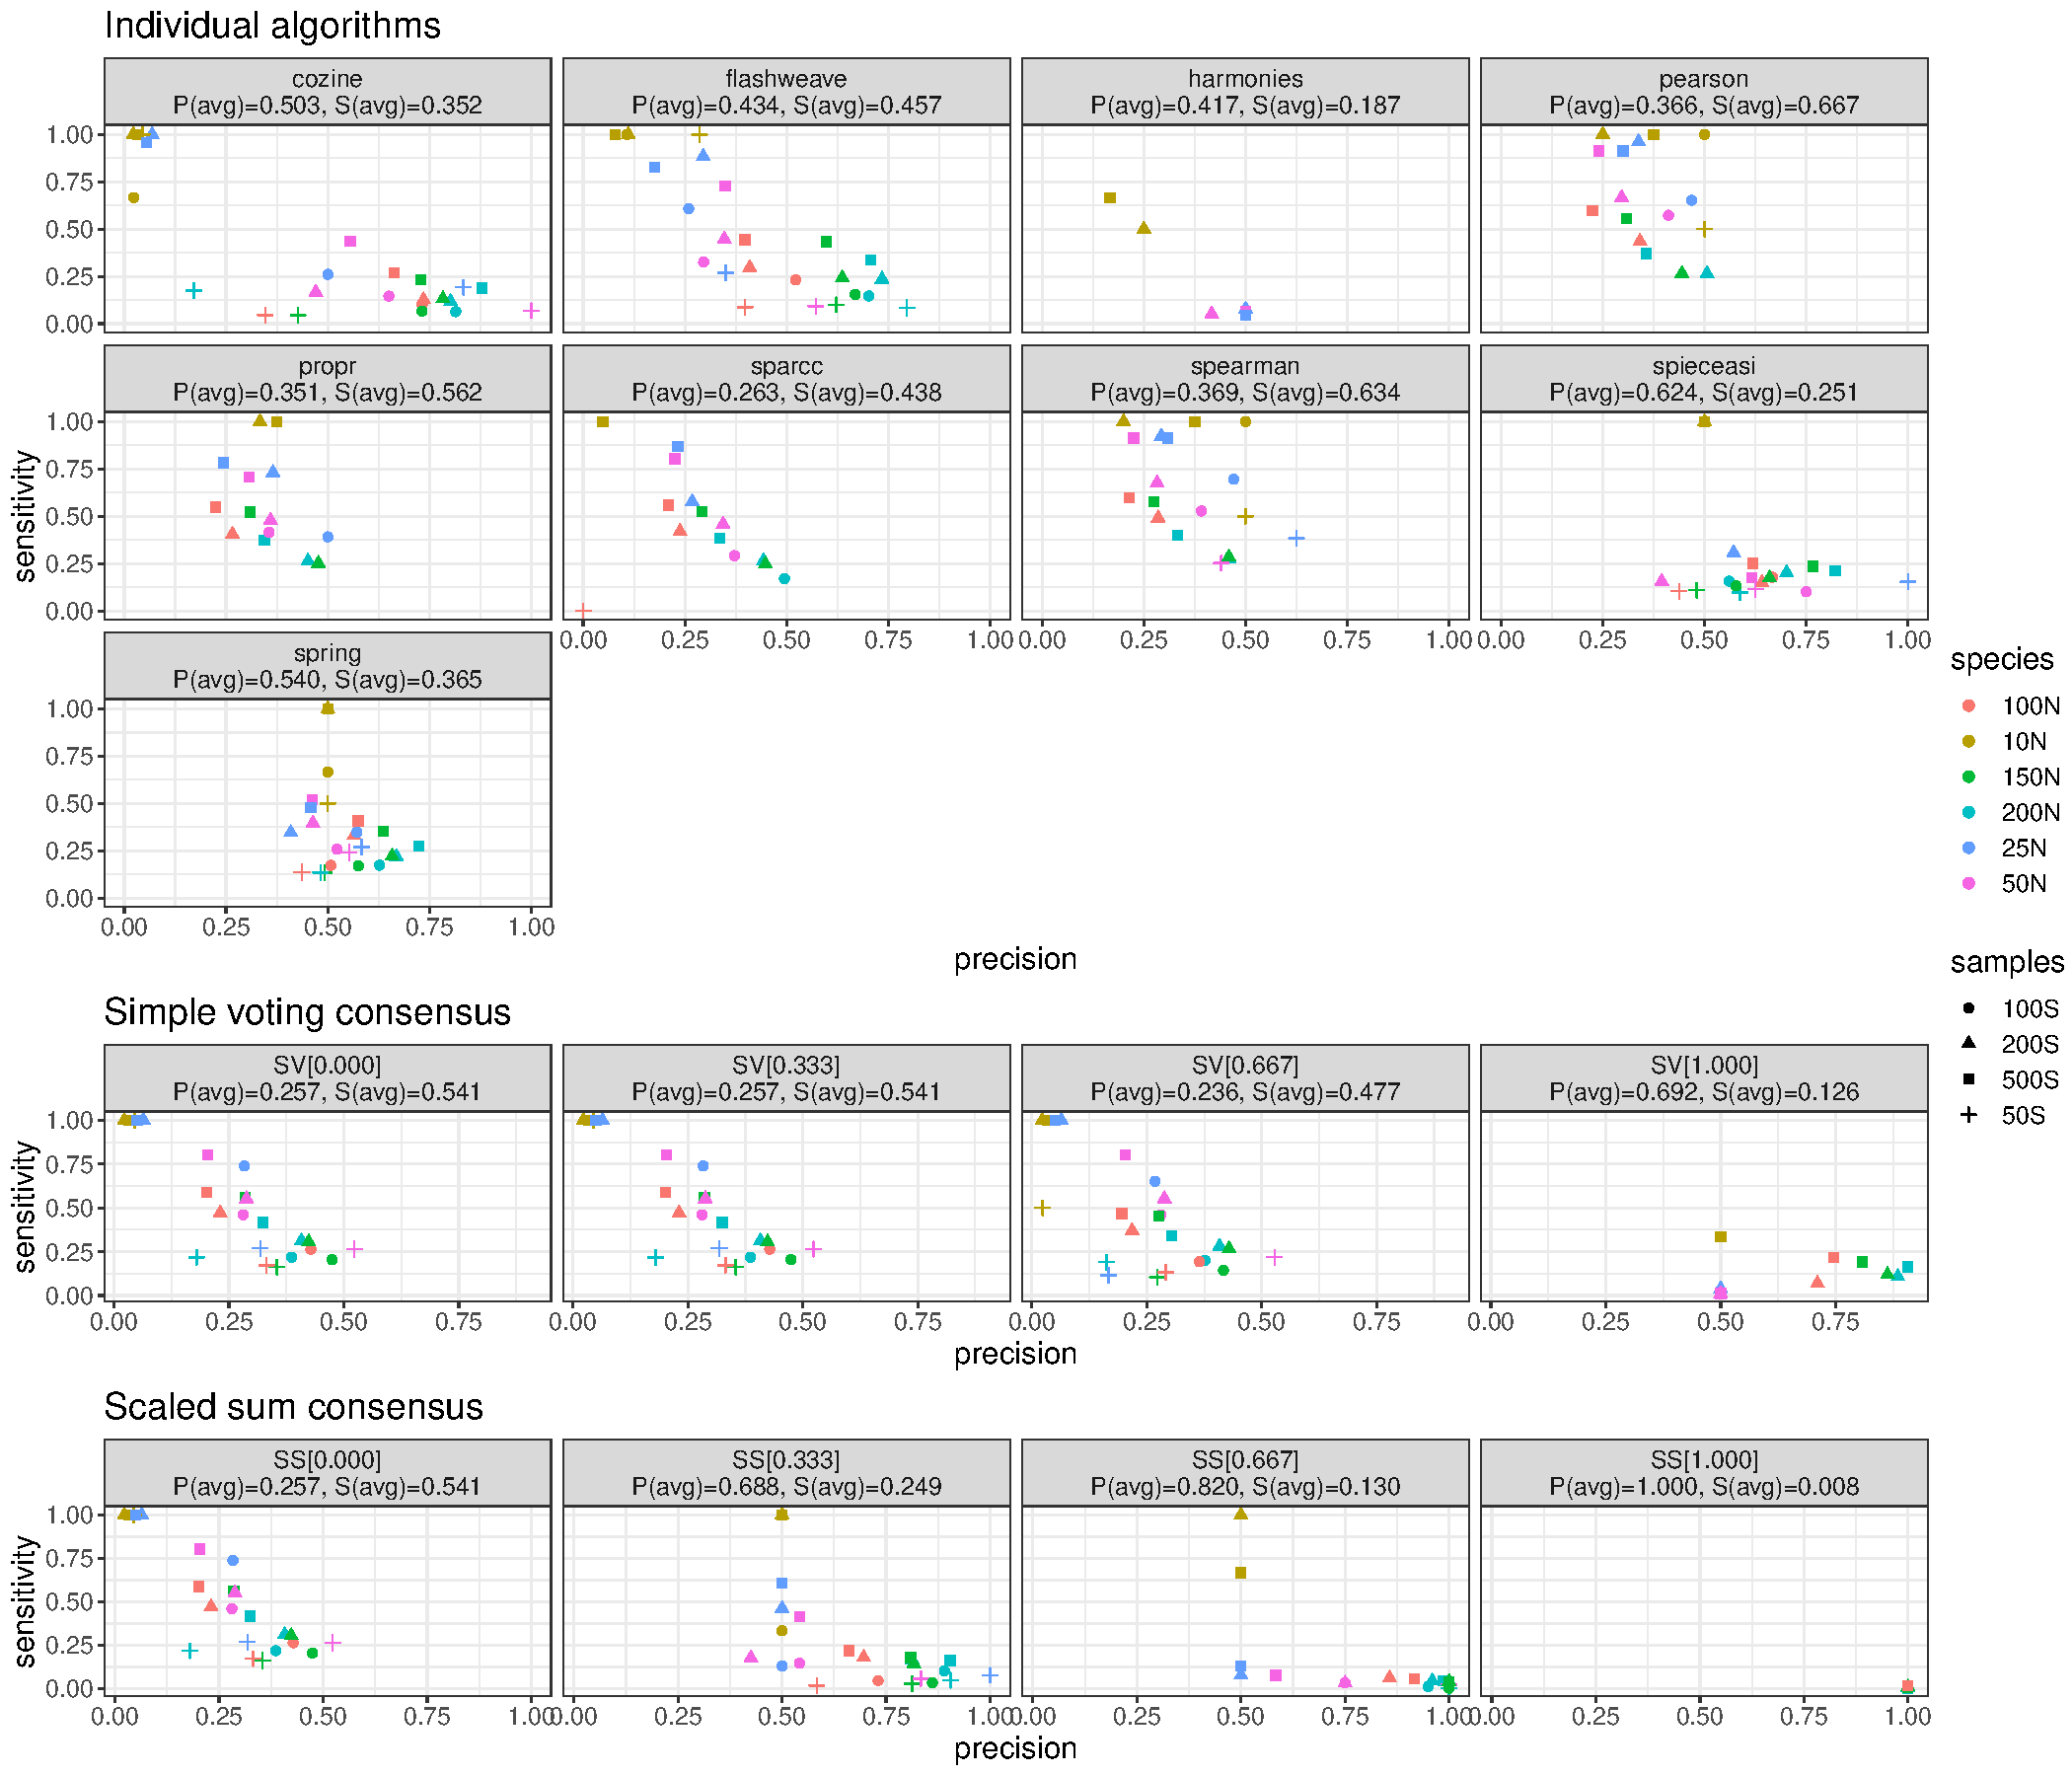
\includegraphics[width=1.0\linewidth]{figure_s6.pdf}
  % \end{figure}
  \begin{figure}[H]
    \centering
      \caption{
        \textbf{The precision and sensitivity of the inferred networks on the ``seqtime'' synthetic interaction data.}
        The different consensus based methods used are: scaled-sum (SS) and simple voting (SV) method.
        Pearson and Spearman methods are not used in the calculation of the consensus.
        Among all the independent network inference methods, \ac{spieceasi} has the best average precision (0.624), but the overall best precision was consistently obtained by the scaled-sum method (0.688, 0.820 and 1.000).
        The simple voting method when using presence of edges in all inferred networks as a requirement ($p = 1.000$), also outperforms \ac{spieceasi} on average precision (0.692).
        These results show that the scaled-sum method is not only much better suited for inferring robust and accurate interactions from count data regardless of the distributions and topologies, but it is also capable of accurately extracting real associations (gLV interactions) from count data.
      }
    \label{fig:figure_s6}
  \end{figure}
  % \FloatBarrier
  % \newpage

  % \begin{figure}[H]
  %   \centering
  %   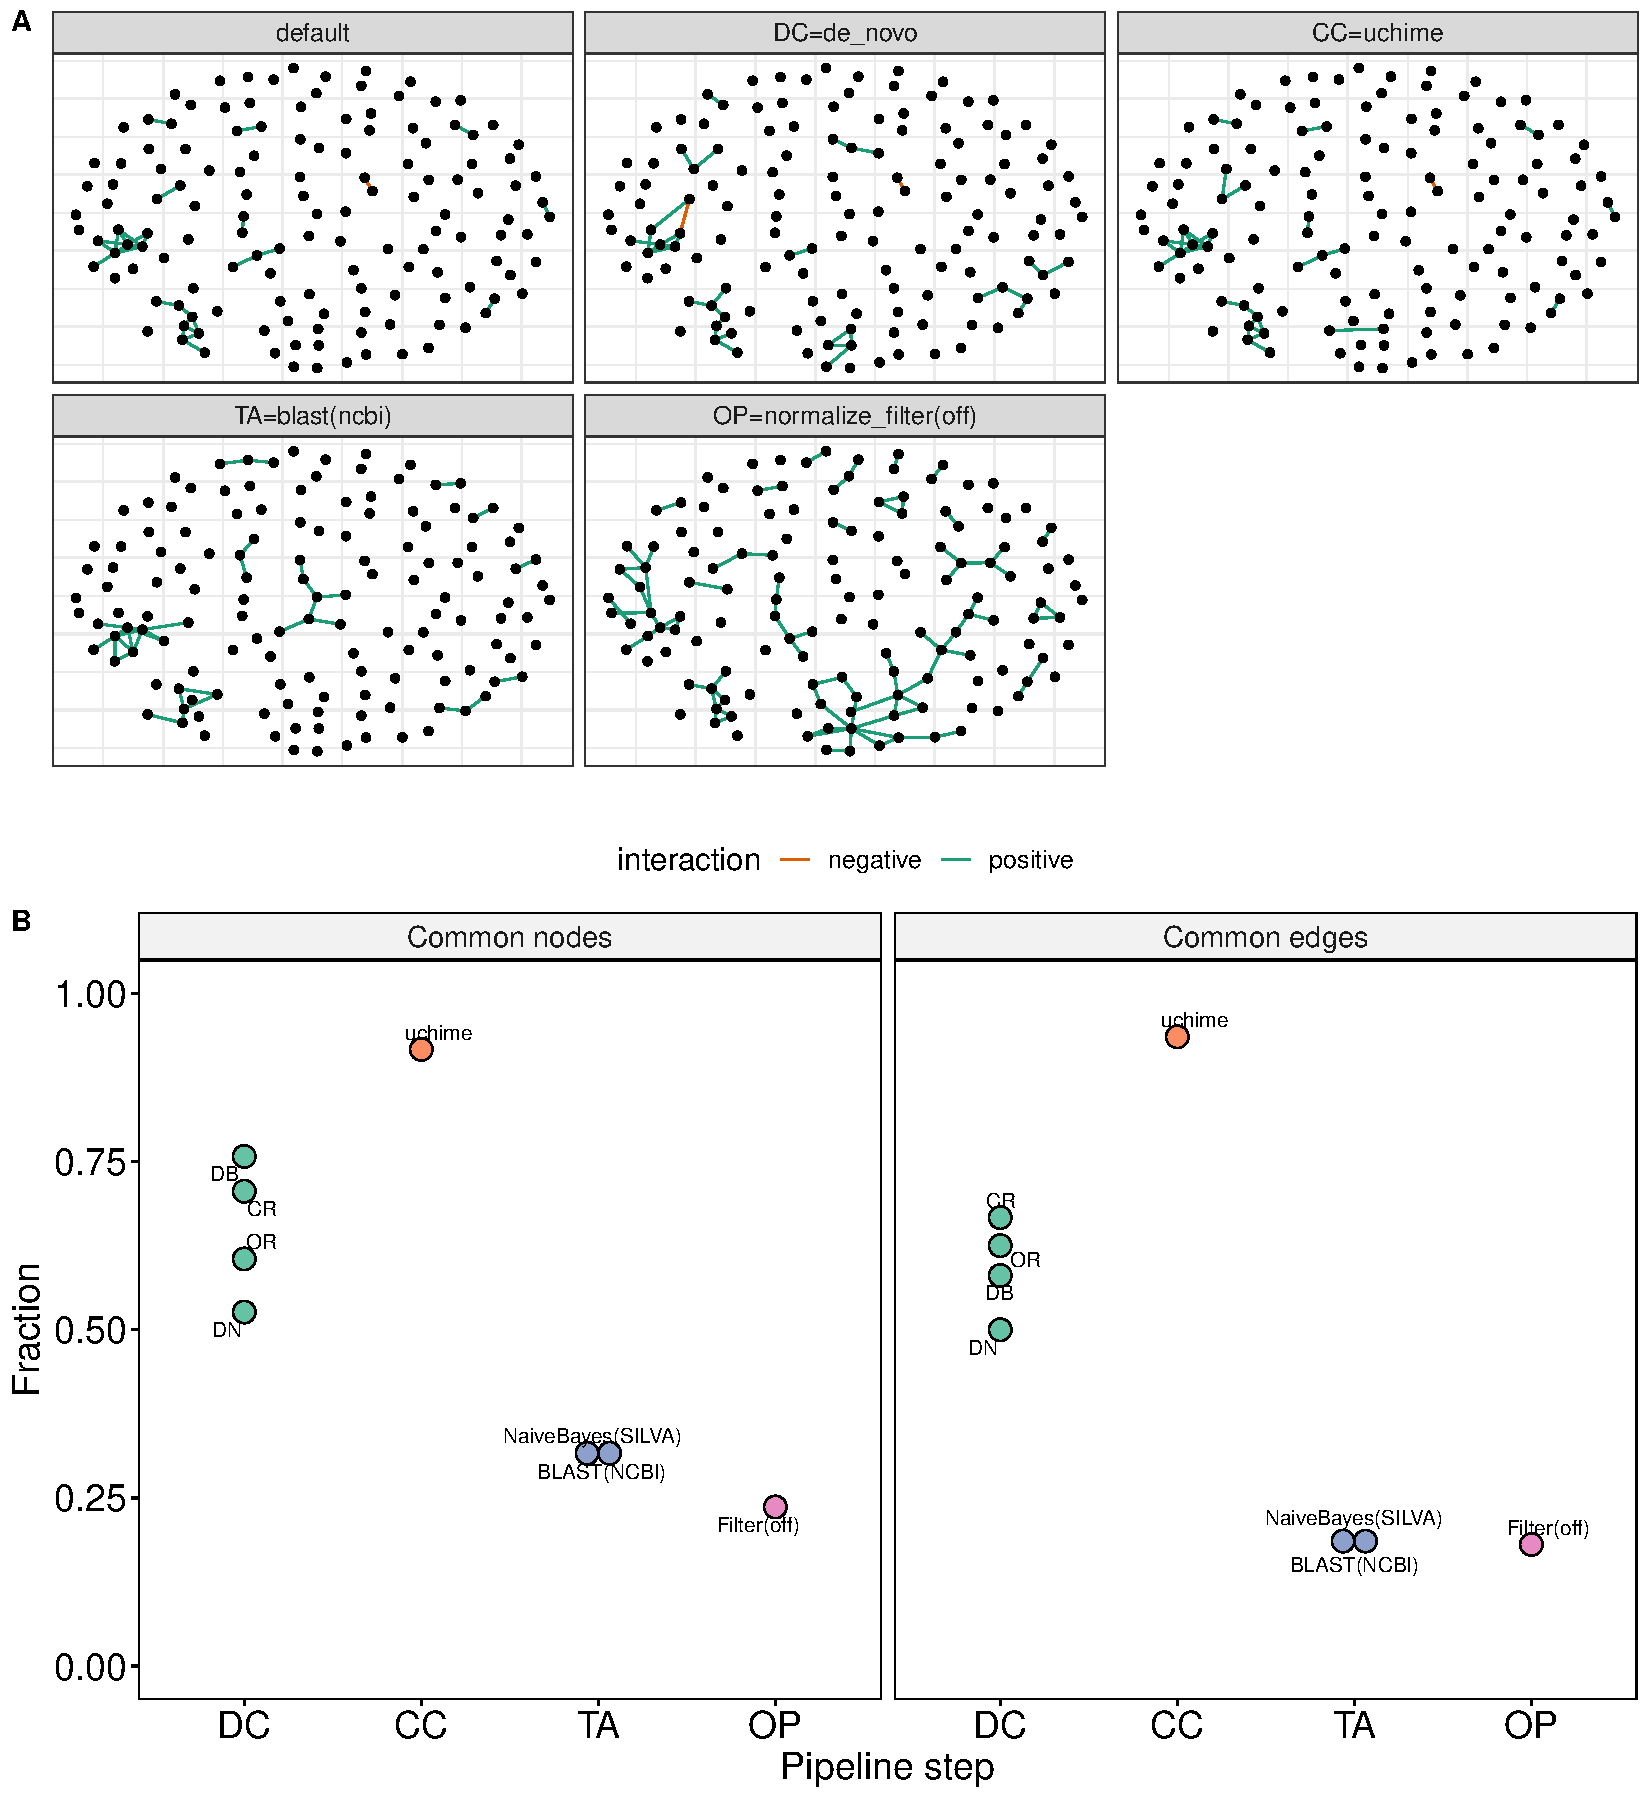
\includegraphics[width=1.0\linewidth]{figure_s7.pdf}
  % \end{figure}
  \begin{figure}[H]
    \centering
    \caption{
      \textbf{Sensitivity analysis of the default settings of the \ac{micone} pipeline}.
      \textbf{(A)} The network constructed using the default pipeline parameters (DC=\ac{dada2}, CC=remove bimera, TA=\ac{gg}, OP=Filter(on), NI=scaled-sum consensus) is compared with networks generated when one of the steps use a different tool.
      The layout is created by fixing the positions of all the nodes from all networks and then drawing only the relevant edges.
      The edges colored green are positive associations and those in red are negative associations.
      We observe that changing the TA and OP steps leads to the creation of the most number of unique edges.
      \textbf{(B)} The dot plot showing the fraction of nodes (left) and edges (right) in common between the default network and the networks generated by changing one step of the default pipeline.
      The low value of the common fraction for TA and OP steps shows that these steps induce the biggest changes nodes and edges.
      The NI step is not shown in this analysis because the consensus method uses edges from the individual network inference methods and a comparison would be biased.
    }
    \label{fig:figure_s7}
  \end{figure}
  % \FloatBarrier
  % \newpage

